\section{Experimental Investigation of Optical Contact Bonding}
\label{sec:optical_contact_bonding}

To evaluate the feasibility and reliability of the sealing process, a series
of optical contact bonding experiments were conducted at the Chemistry
Department of the University of Bari (UniBa), Italy. The samples utilized for
these tests were fused silica disks with a diameter of \SI{4}{\centi\meter},
characterized by a total thickness variation (TTV) of
\textbf{[PLACEHOLDER]} and an average surface roughness ($R_a$) of
\textbf{[PLACEHOLDER]}. 

\subsection{Cleaning Protocols and Surface Activation}
To achieve successful optical contact, the surfaces must be exceptionally
clean and highly hydrophilic. It is critical to emphasize that these
experiments were conducted outside of a dedicated cleanroom environment. The
absence of a strictly controlled, particle-free atmosphere introduces a
significant degree of environmental randomness and variability to the trials.
Because the bonding mechanism relies on short-range intermolecular forces, even
microscopic airborne dust particles or contaminants can become trapped between
the substrates, creating localized voids and completely preventing the
spontaneous propagation of the bonding wave.

Several cleaning and activation protocols were evaluated to mitigate this
environmental limitation and determine the most robust preparation strategy.

\paragraph{Baseline Ethanol Procedure.}
The initial trial consisted of a simple, rapid soaking sequence. The disks
were immersed in ethanol, immediately followed by a quick soak in deionized
water (DIW). The samples were subsequently dried by vigorously shaking them
for a few seconds. Out of the pairs prepared with this rudimentary method,
only two successfully bonded. Following this initial test, all subsequent
procedures were strictly performed under a chemical hood utilizing an
ultrasonic cleaner to ensure proper contamination removal
(Figure~\ref{fig:hood_setup}).

\begin{figure}[htbp]
    \centering
    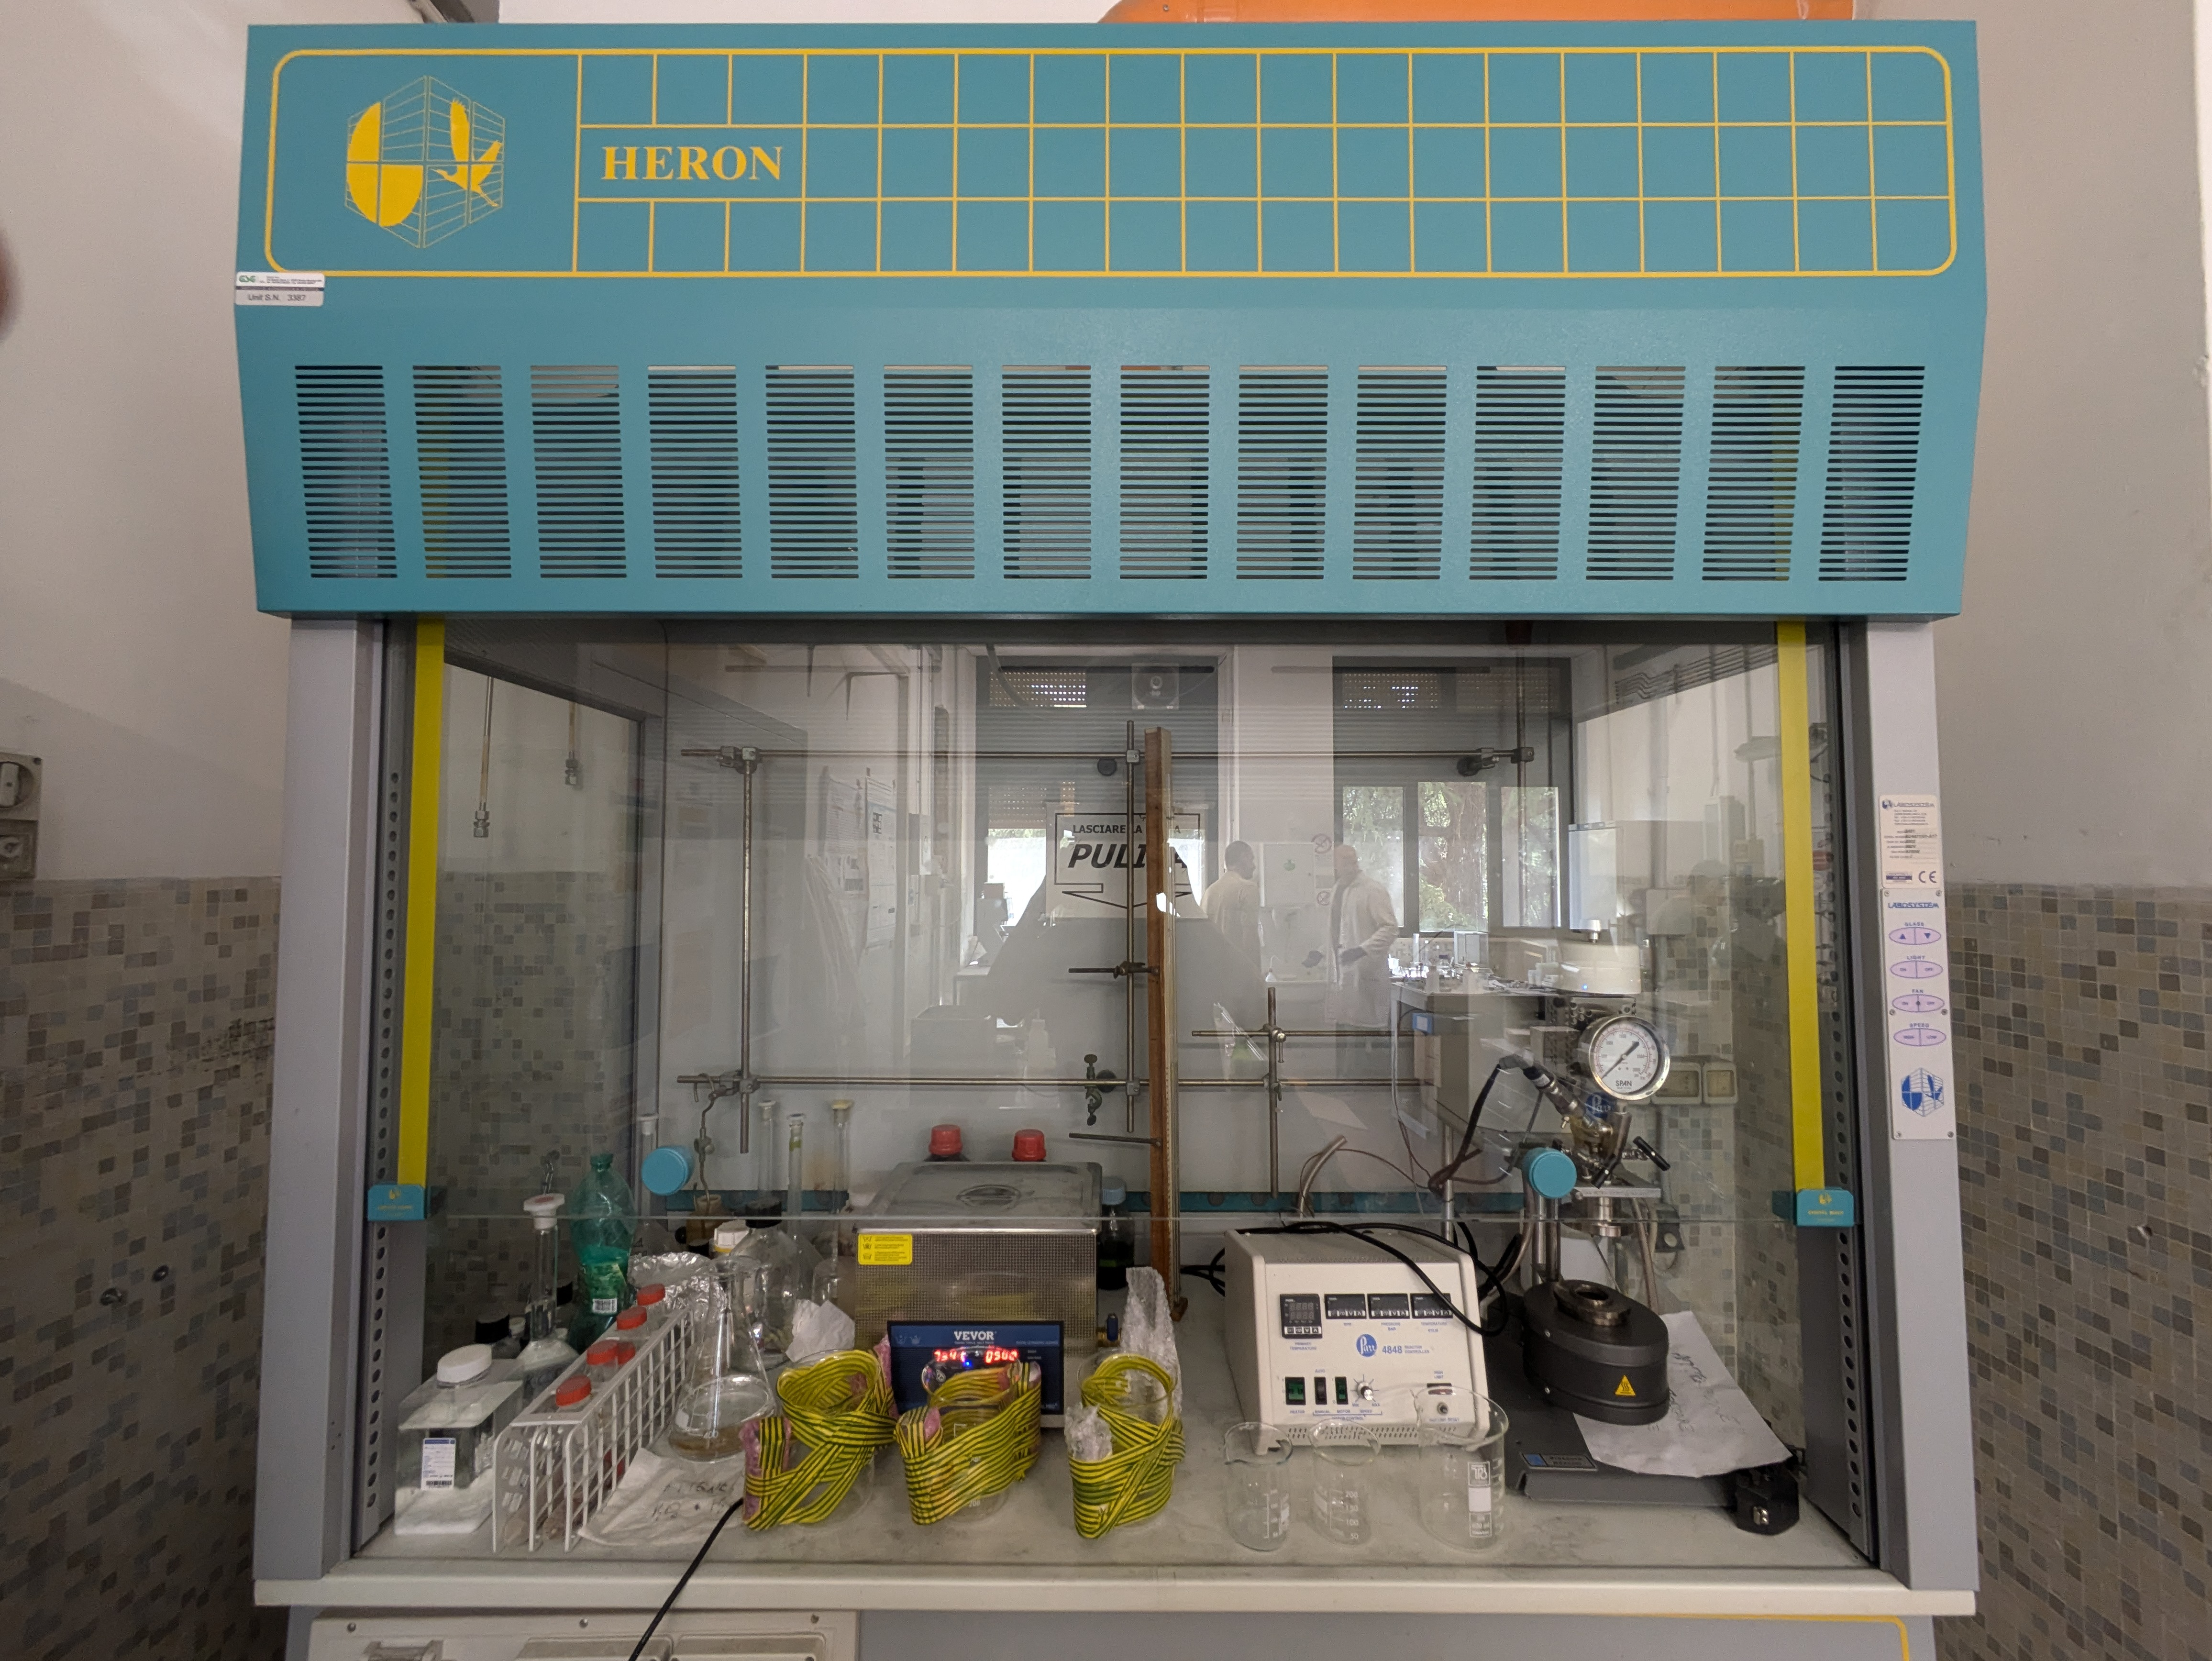
\includegraphics[width=0.6\linewidth]{Images/chemical_hood.jpeg}
    \caption{Experimental setup at UniBa, showing the chemical hood and the
    ultrasonic cleaner utilized for the controlled cleaning protocols.}
    \label{fig:hood_setup}
\end{figure}

\paragraph{Plasma-Only Procedure.}
The first controlled protocol relied exclusively on plasma activation. The
disks were lightly washed with an acetone and DIW mixture before being
immediately transferred into an \ce{O2} plasma system (700~\text{mTorr},
\SI{30}{\watt} RF power). Various exposure times ranging from 1 to 10 minutes
were investigated. It was observed that both \SI{5}{\minute} and
\SI{10}{\minute} exposures provided sufficient surface activation for bonding.
Under the 10-minute plasma configuration, two out of the three tested pairs
successfully bonded, while the 5-minute exposure also yielded a successfully
bonded pair (Figure~\ref{fig:plasma_treatment}).

\begin{figure}[htbp]
    \centering
    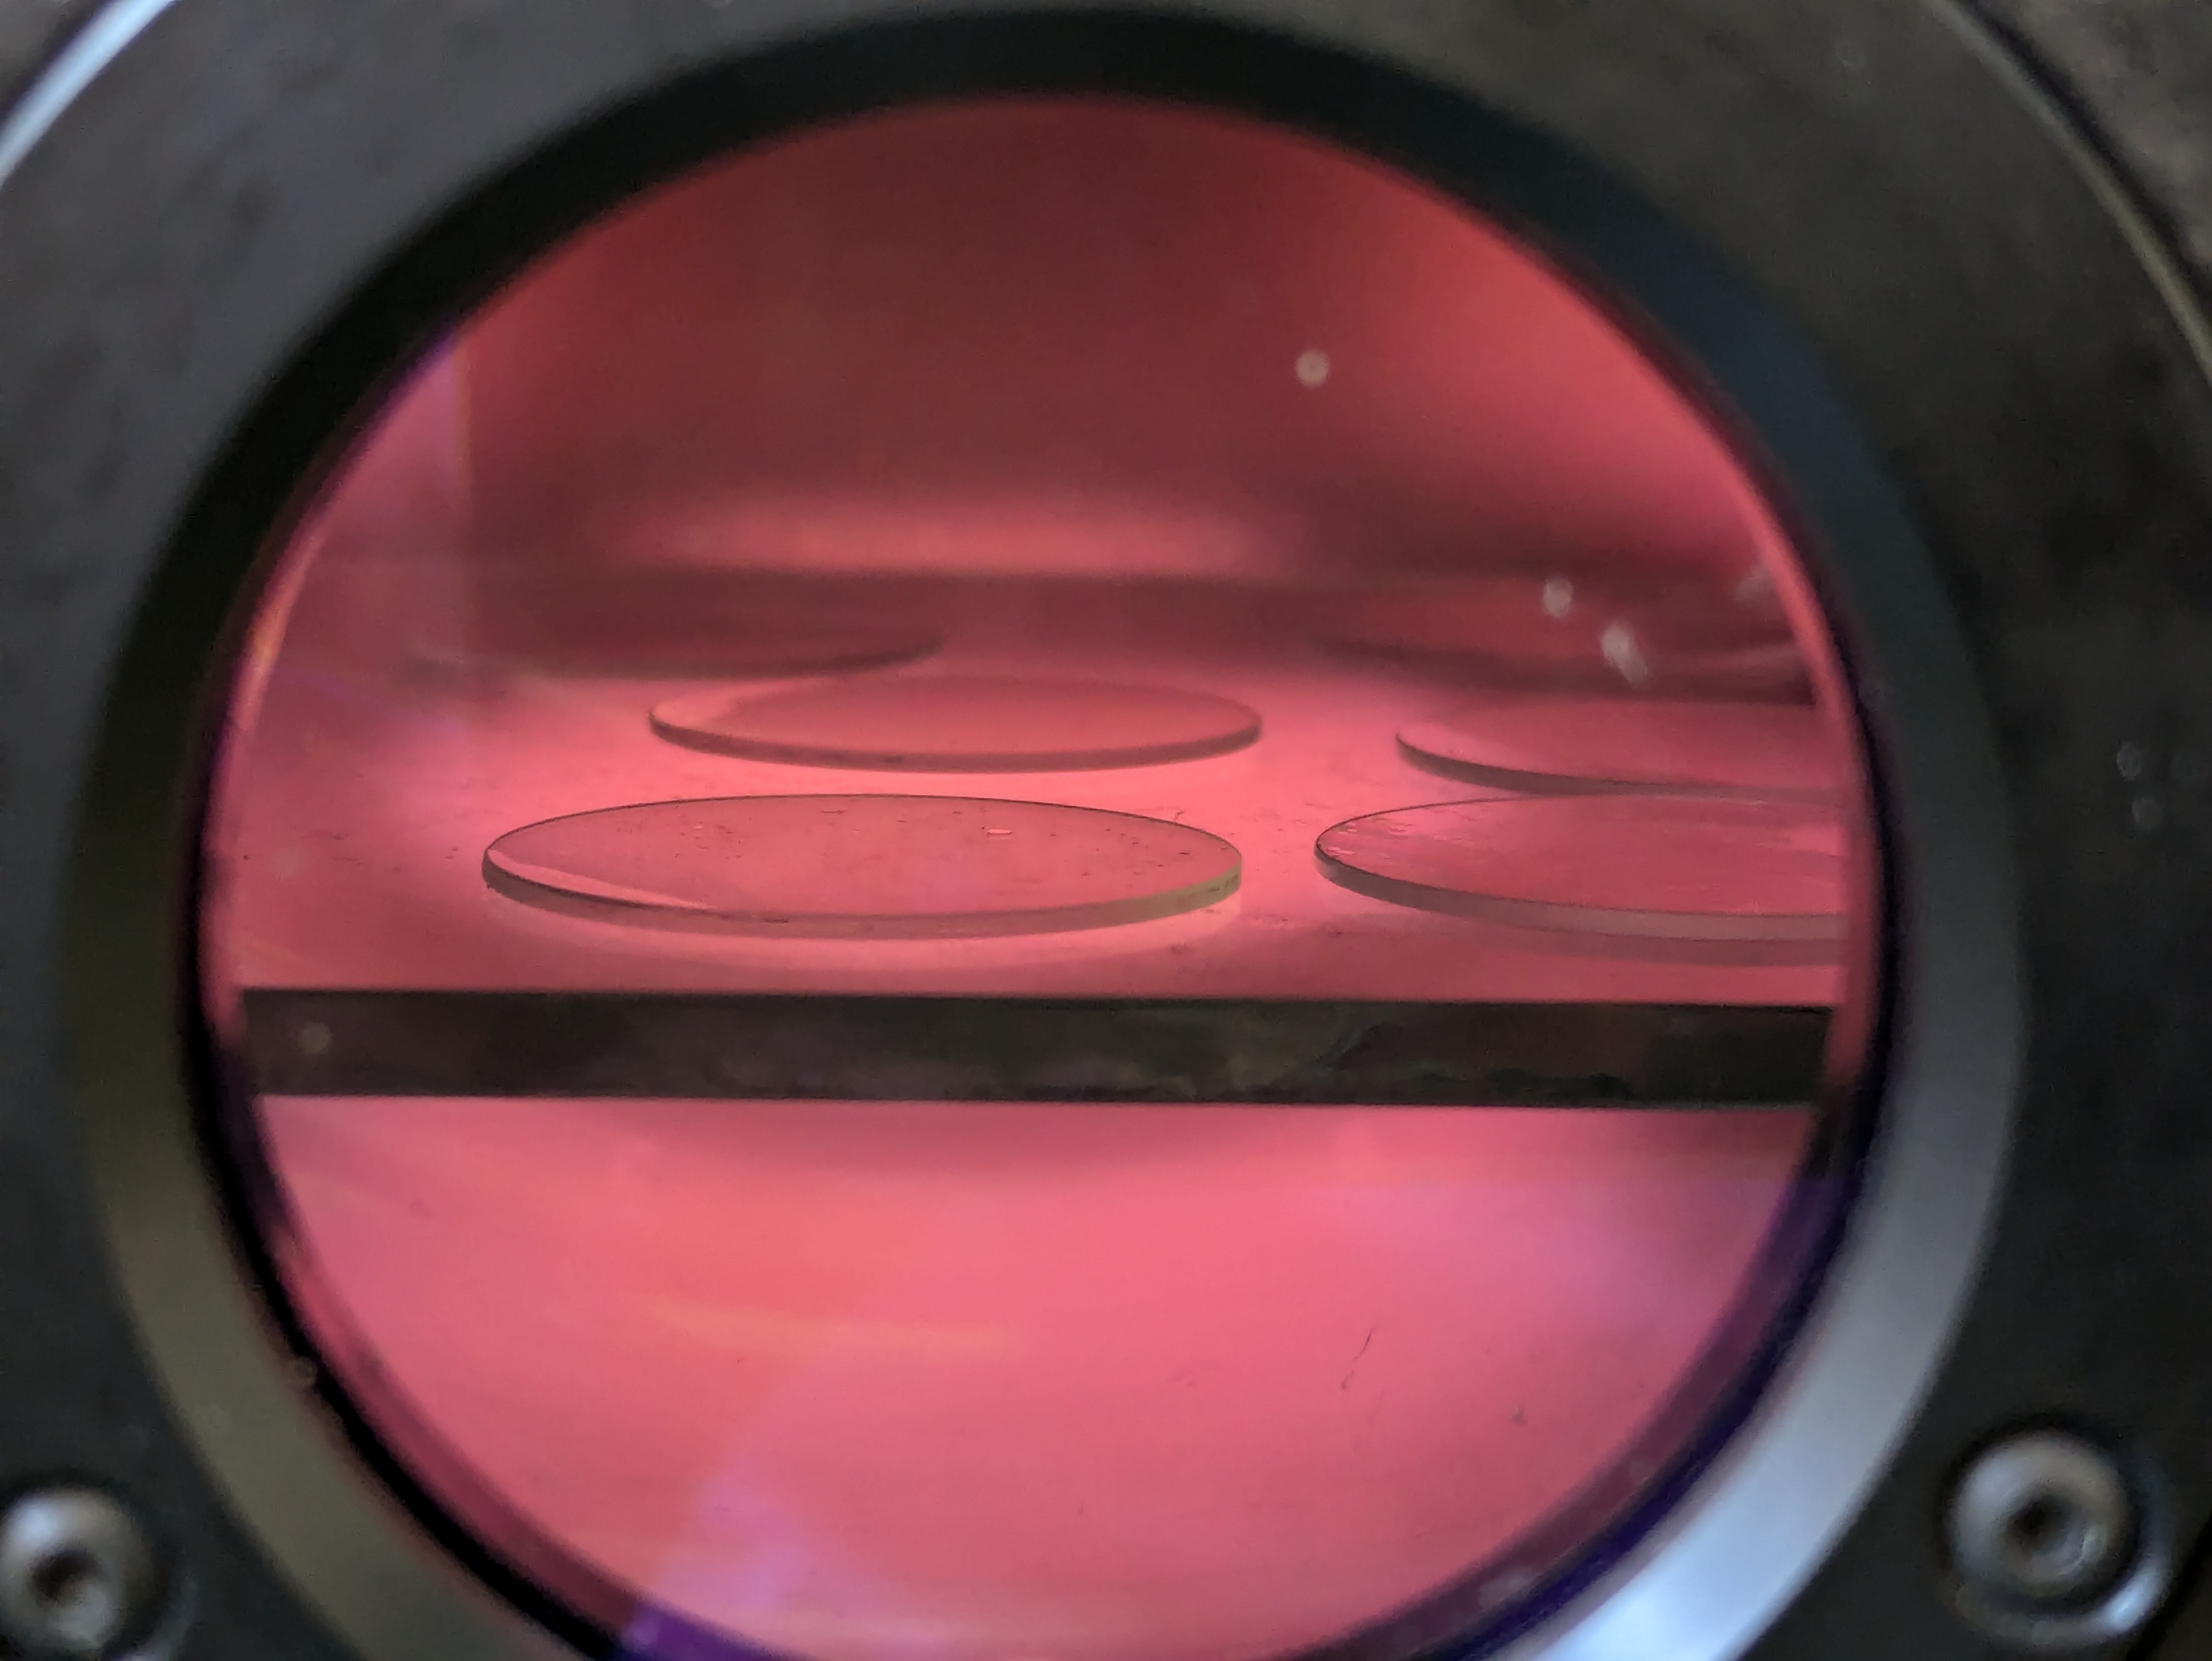
\includegraphics[width=0.5\linewidth]{Images/plasmapurple.jpeg}
    \caption{Oxygen (\ce{O2}) plasma treatment of the fused silica disks.
    The activated plasma gas imparts a characteristic purple glow to the
    interior of the vacuum chamber during the surface modification process.}
    \label{fig:plasma_treatment}
\end{figure}
\paragraph{Piranha Solution Procedure.}
A chemical-based activation approach was also tested. The disks were first
soaked in DIW for 2 minutes, followed by a 20-minute immersion in a piranha
solution (\ce{H2SO4}:\ce{H2O2} in a 3:1 ratio) heated to \SI{70}{\celsius}.
This aggressively removes organic residues and hydroxylates the silica
surface. After the piranha bath, the disks were soaked in DIW for 5 minutes
to eliminate any acidic residues and were extensively dried using a
high-pressure \ce{N2} gun (Figure~\ref{fig:n2_gun}).

\begin{figure}[htbp]
    \centering
    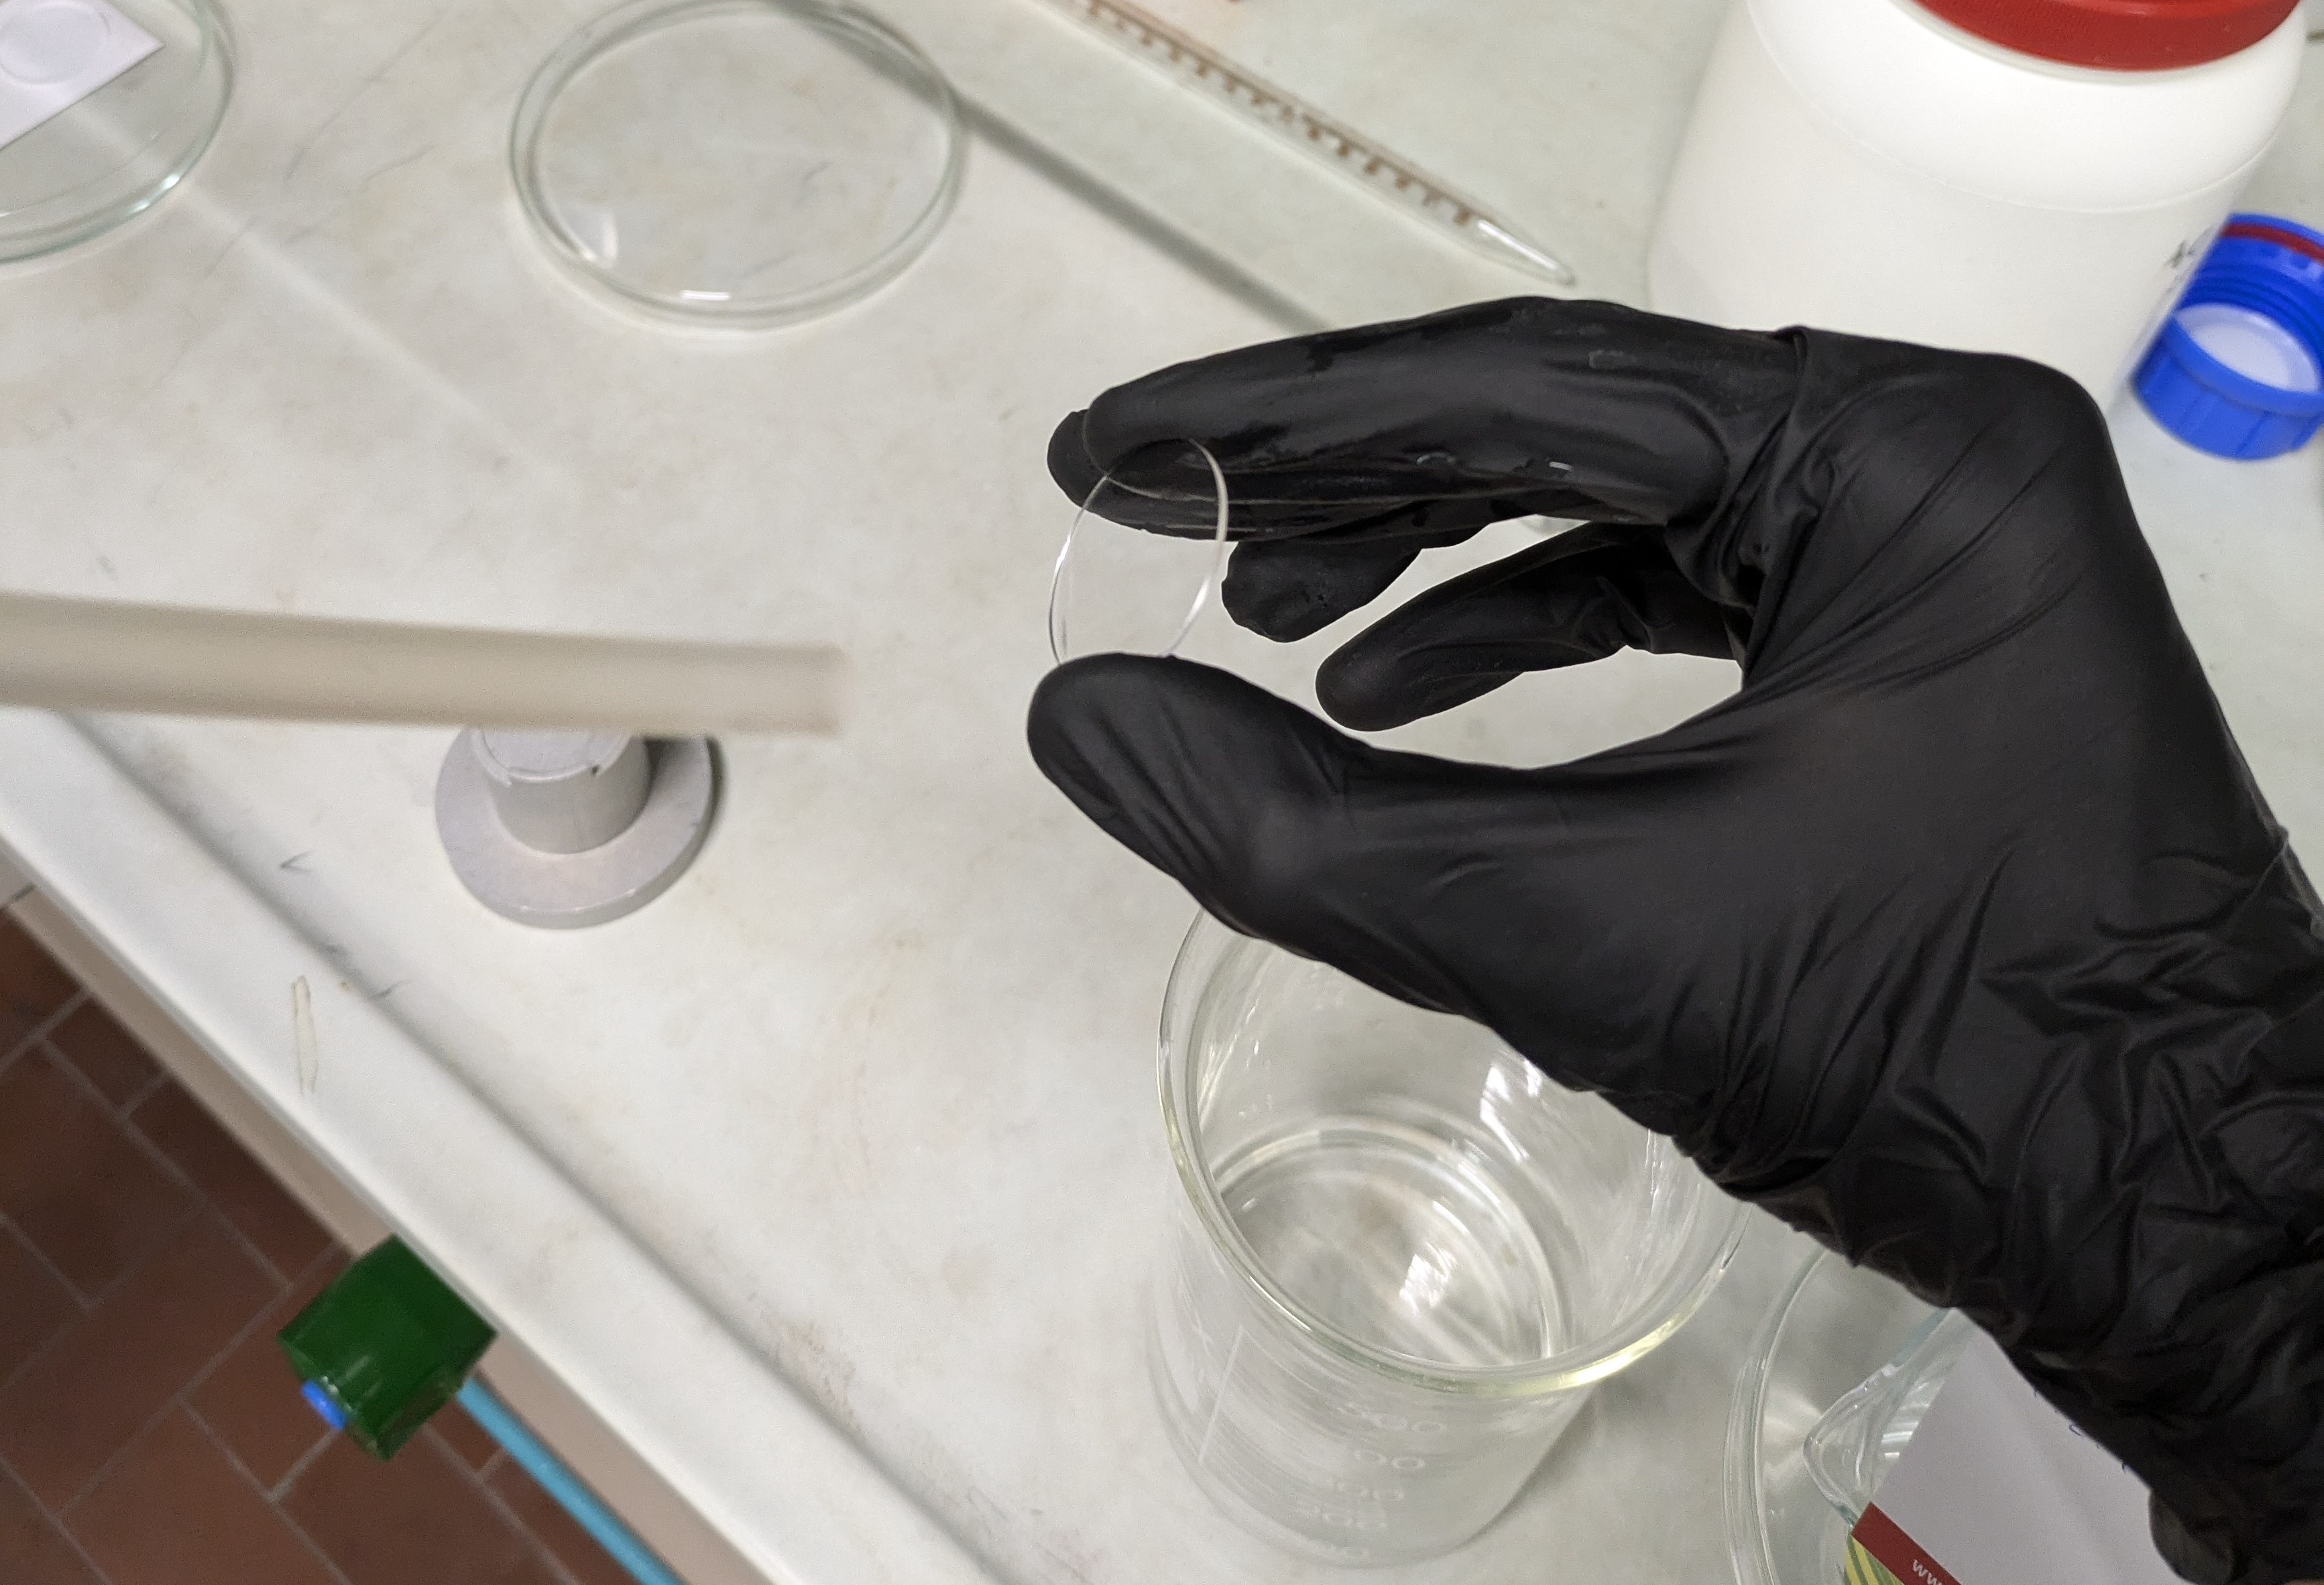
\includegraphics[width=0.5\linewidth]{Images/n2drying.png}
    \caption{Extensive drying of the fused silica disks utilizing a high-pressure
    nitrogen (\ce{N2}) gun to prevent water mark formation.}
    \label{fig:n2_gun}
\end{figure}

\paragraph{Sequential RCA-1 and Piranha Procedure.}
A multi-step chemical protocol was also evaluated to leverage both particle
removal and strong oxidation. The disks were rinsed with DIW and then
immersed in an RCA-1 solution for \SI{10}{\minute} at \SI{70}{\celsius} to
strip organic contaminants and particles. Following another DIW rinse, the
samples were treated with a piranha solution for \SI{10}{\minute} at
\SI{70}{\celsius} to further hydroxylate the surface. Finally, after a
thorough 5-minute DIW rinse to remove acid traces, the disks were dried using
the high-pressure \ce{N2} gun. Three pairs were processed using this complete
wet-chemical sequence, and all three successfully achieved bonding.

\paragraph{Combined Piranha and Plasma Procedure.}
The final protocol integrated both chemical and physical activation methods.
The disks underwent the exact same 20-minute piranha treatment and \ce{N2}
drying step, but this was immediately followed by a 10-minute \ce{O2} plasma
activation (700~\text{mTorr}, \SI{30}{\watt}). The 10-minute duration
was explicitly selected based on the previous plasma-only results, which
demonstrated optimal bonding reliability at this longer exposure time.

\subsection{Contacting and Curing}
Regardless of the cleaning protocol applied, the physical contacting step was
identical for all samples. The treated disks were brought into contact using
a custom-designed alignment fixture (Figure~\ref{fig:holding_piece}) and were
subsequently pressed firmly by hand for approximately one minute to initiate
the spontaneous bonding wave.

\begin{figure}[htbp]
    \centering
    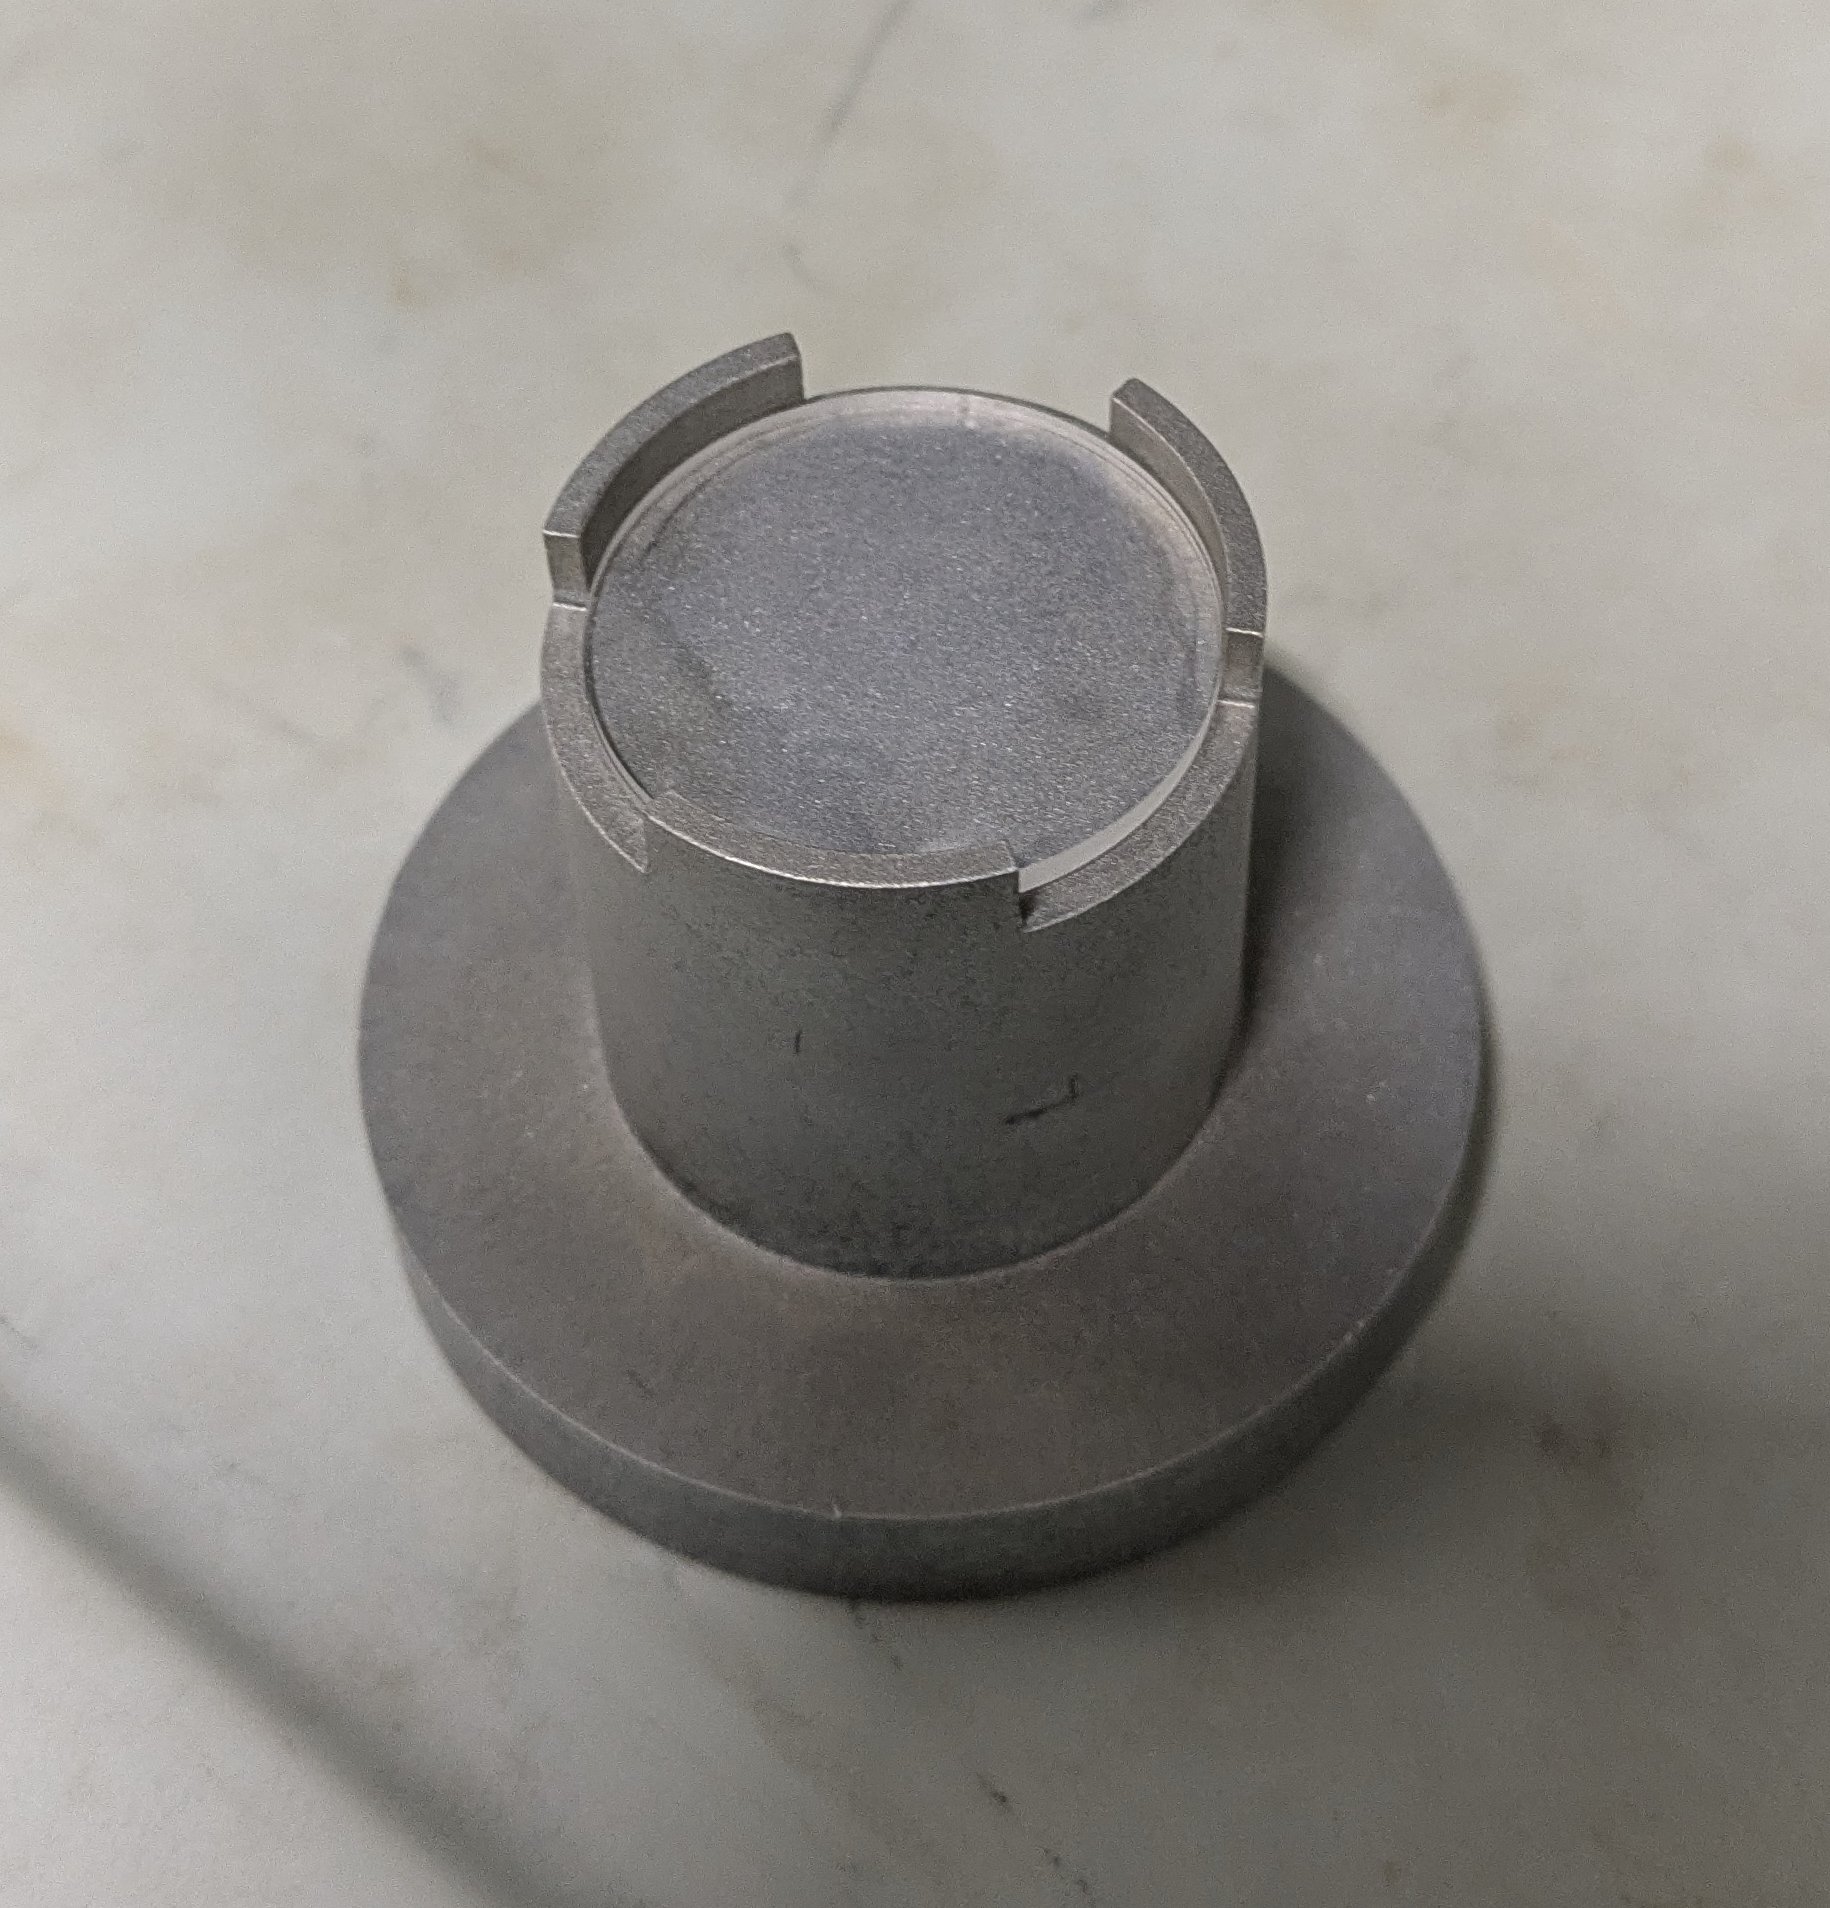
\includegraphics[width=0.5\linewidth]{Images/bonder.png}
    \caption{Alignment fixture utilized to accurately position and hold the
    fused silica disks during the manual pressing phase.}
    \label{fig:holding_piece}
\end{figure}

In standard optical contact bonding, a high-temperature annealing step is
usually performed to convert the weak hydrogen bonds into strong, permanent
covalent siloxane bridges. However, whenever the bonded disks were placed in
the available oven for annealing, complete debonding was observed after a few
hours. This failure was attributed to an excessively steep temperature ramp
rate. If the temperature rises too rapidly, the interfacial water trapped
between the disks evaporates and turns into steam faster than it can diffuse
towards the outer edges. This generates a massive internal pressure that
forces the disks apart. Lacking access to an oven capable of highly
controlled, slow thermal ramping, the high-temperature annealing step was
discarded. Instead, the contacted pairs were left to cure at room temperature
for several days.

\subsection{Results and Image Analysis}
To quantify the efficacy of the different surface treatments despite the
non-cleanroom environment, the bonded samples were optically inspected and
analyzed using the Fiji (ImageJ) software suite. By processing the raw optical
photographs into high-contrast binary maps, the precise percentage of the
successfully bonded area versus the void area was calculated.

Figures~\ref{fig:bonding_results_1} and \ref{fig:bonding_results_2} present
the side-by-side comparison for each evaluated protocol, pairing the raw
optical photograph (left) with its corresponding Fiji-processed binary
image (right).

\begin{figure}[htbp]
    \centering
    % Pair 1: Baseline Ethanol
    \begin{subfigure}{0.45\linewidth}
        \centering
        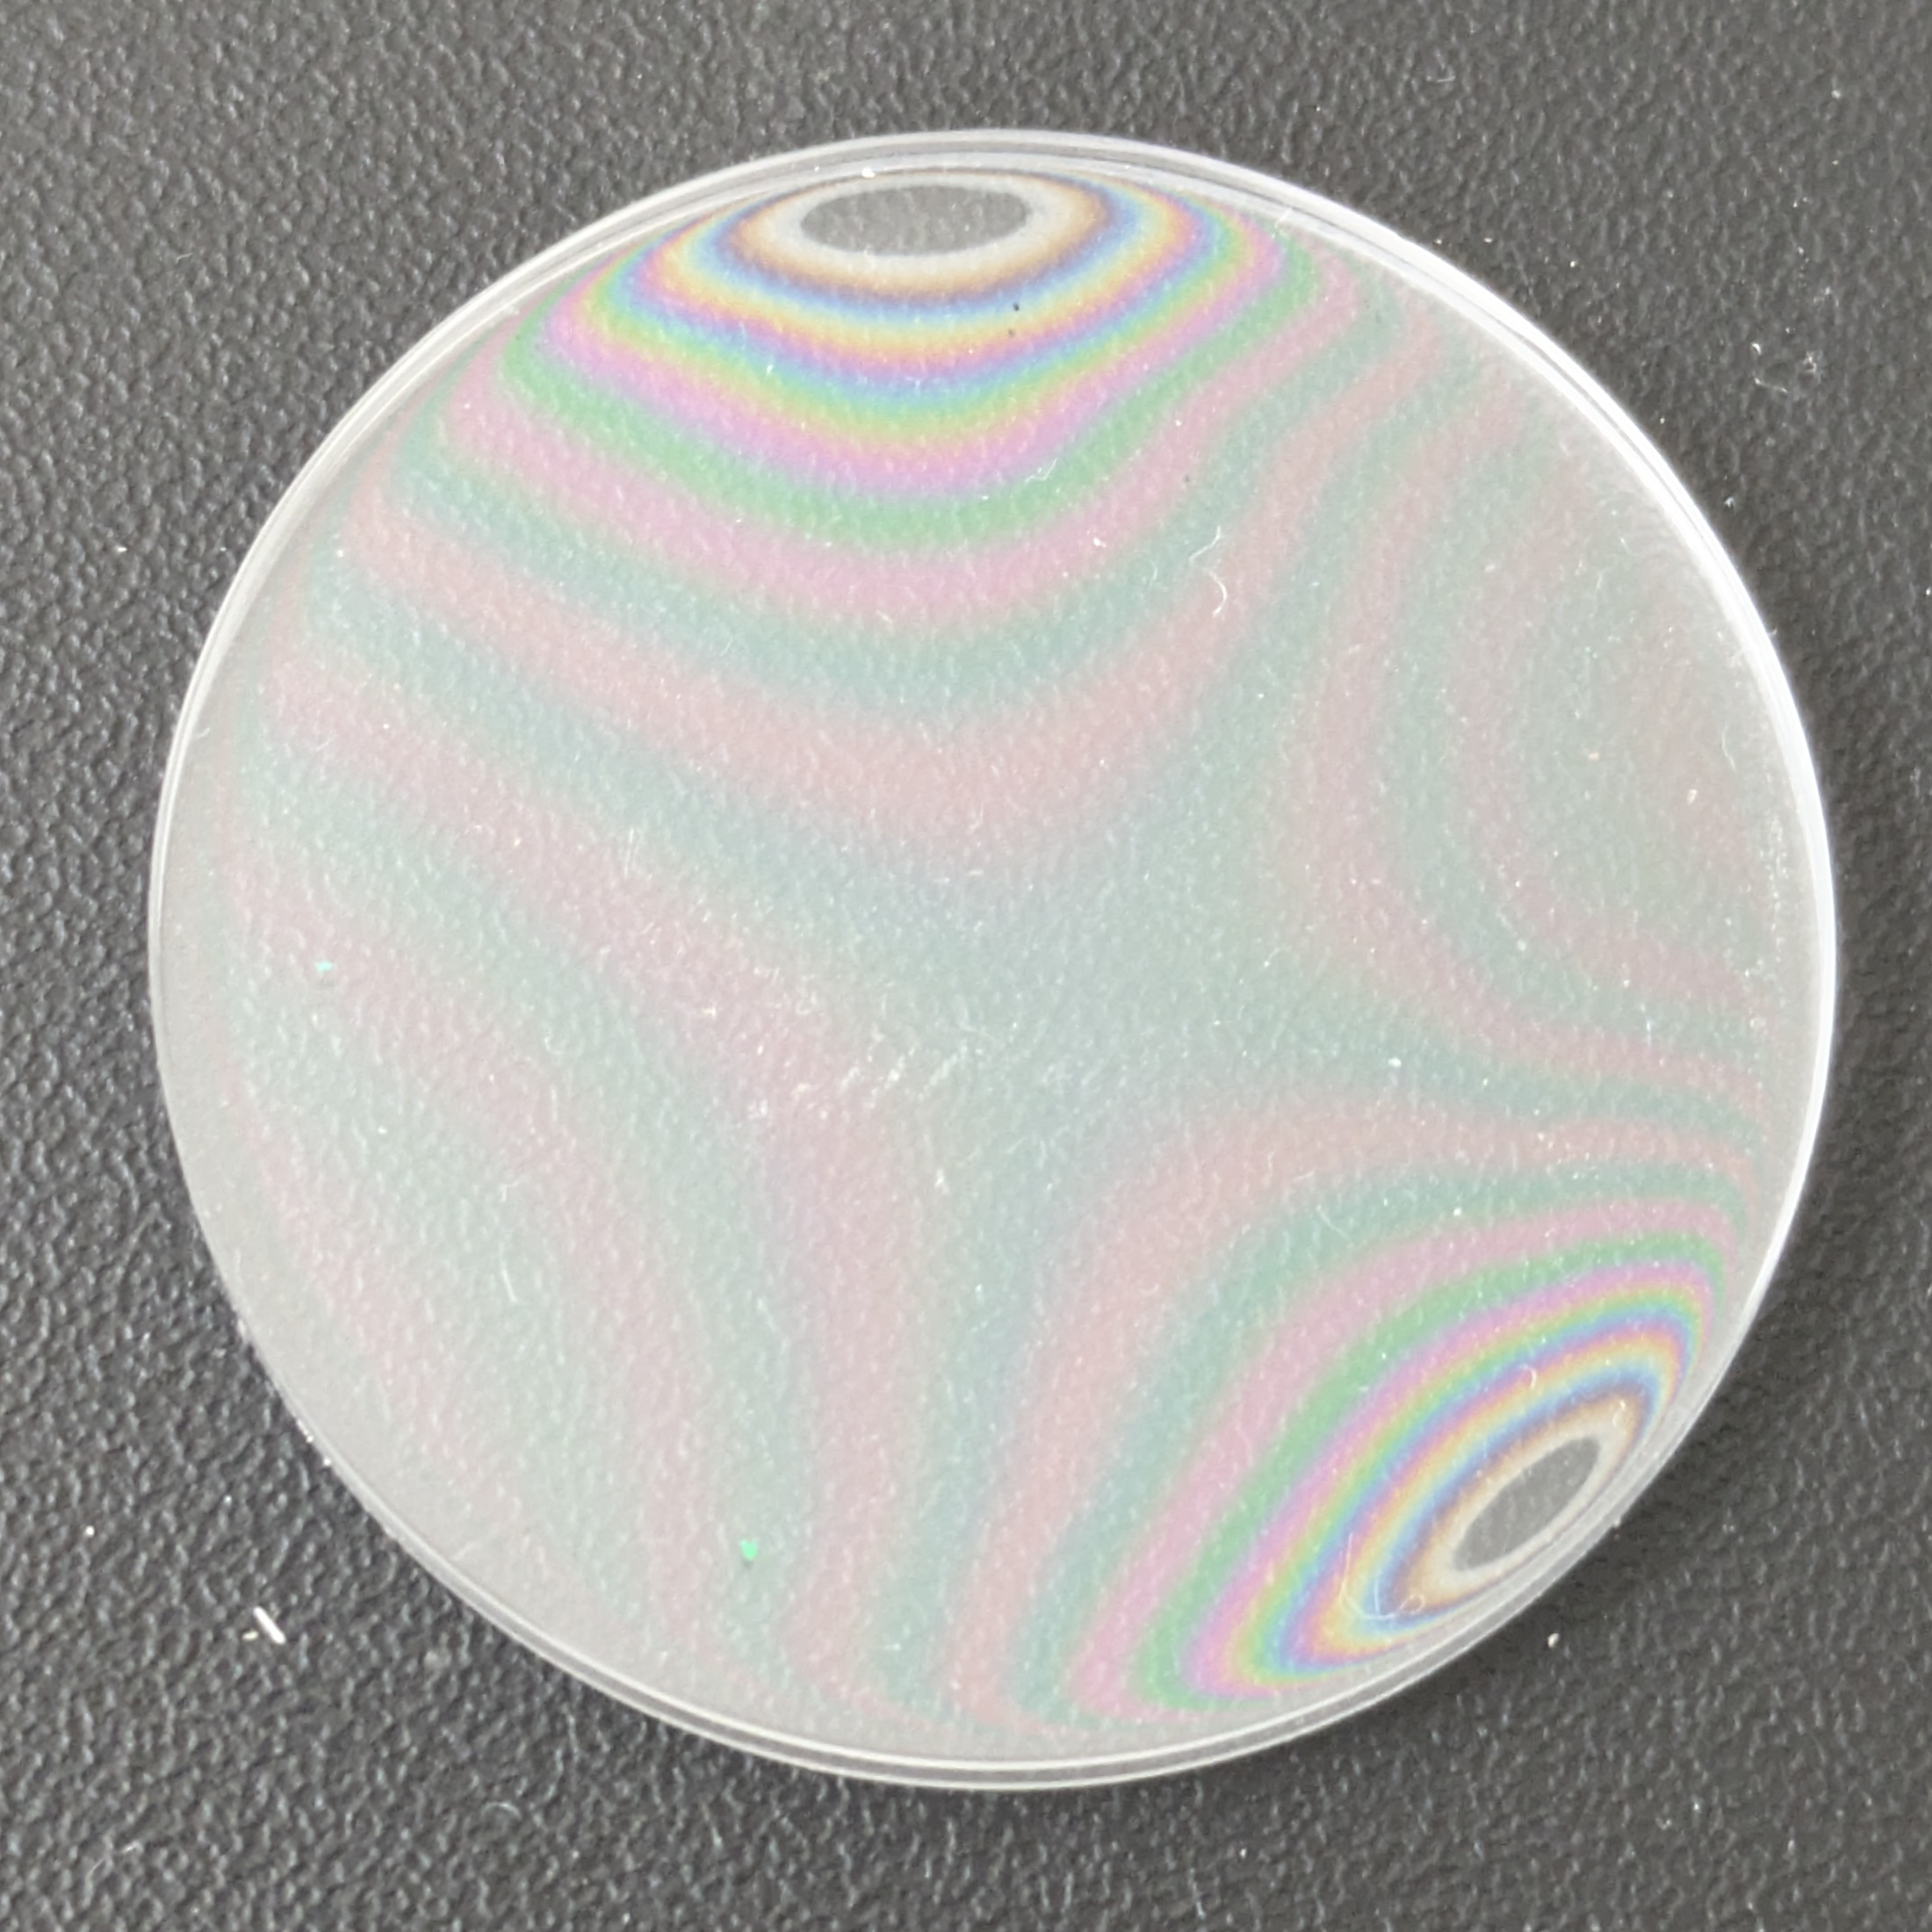
\includegraphics[width=\linewidth]{Images/Disks/Raw/acetone.png}
        \caption{Baseline Ethanol: Raw photograph.}
        \label{fig:eth_raw}
    \end{subfigure}
    \hfill
    \begin{subfigure}{0.45\linewidth}
        \centering
        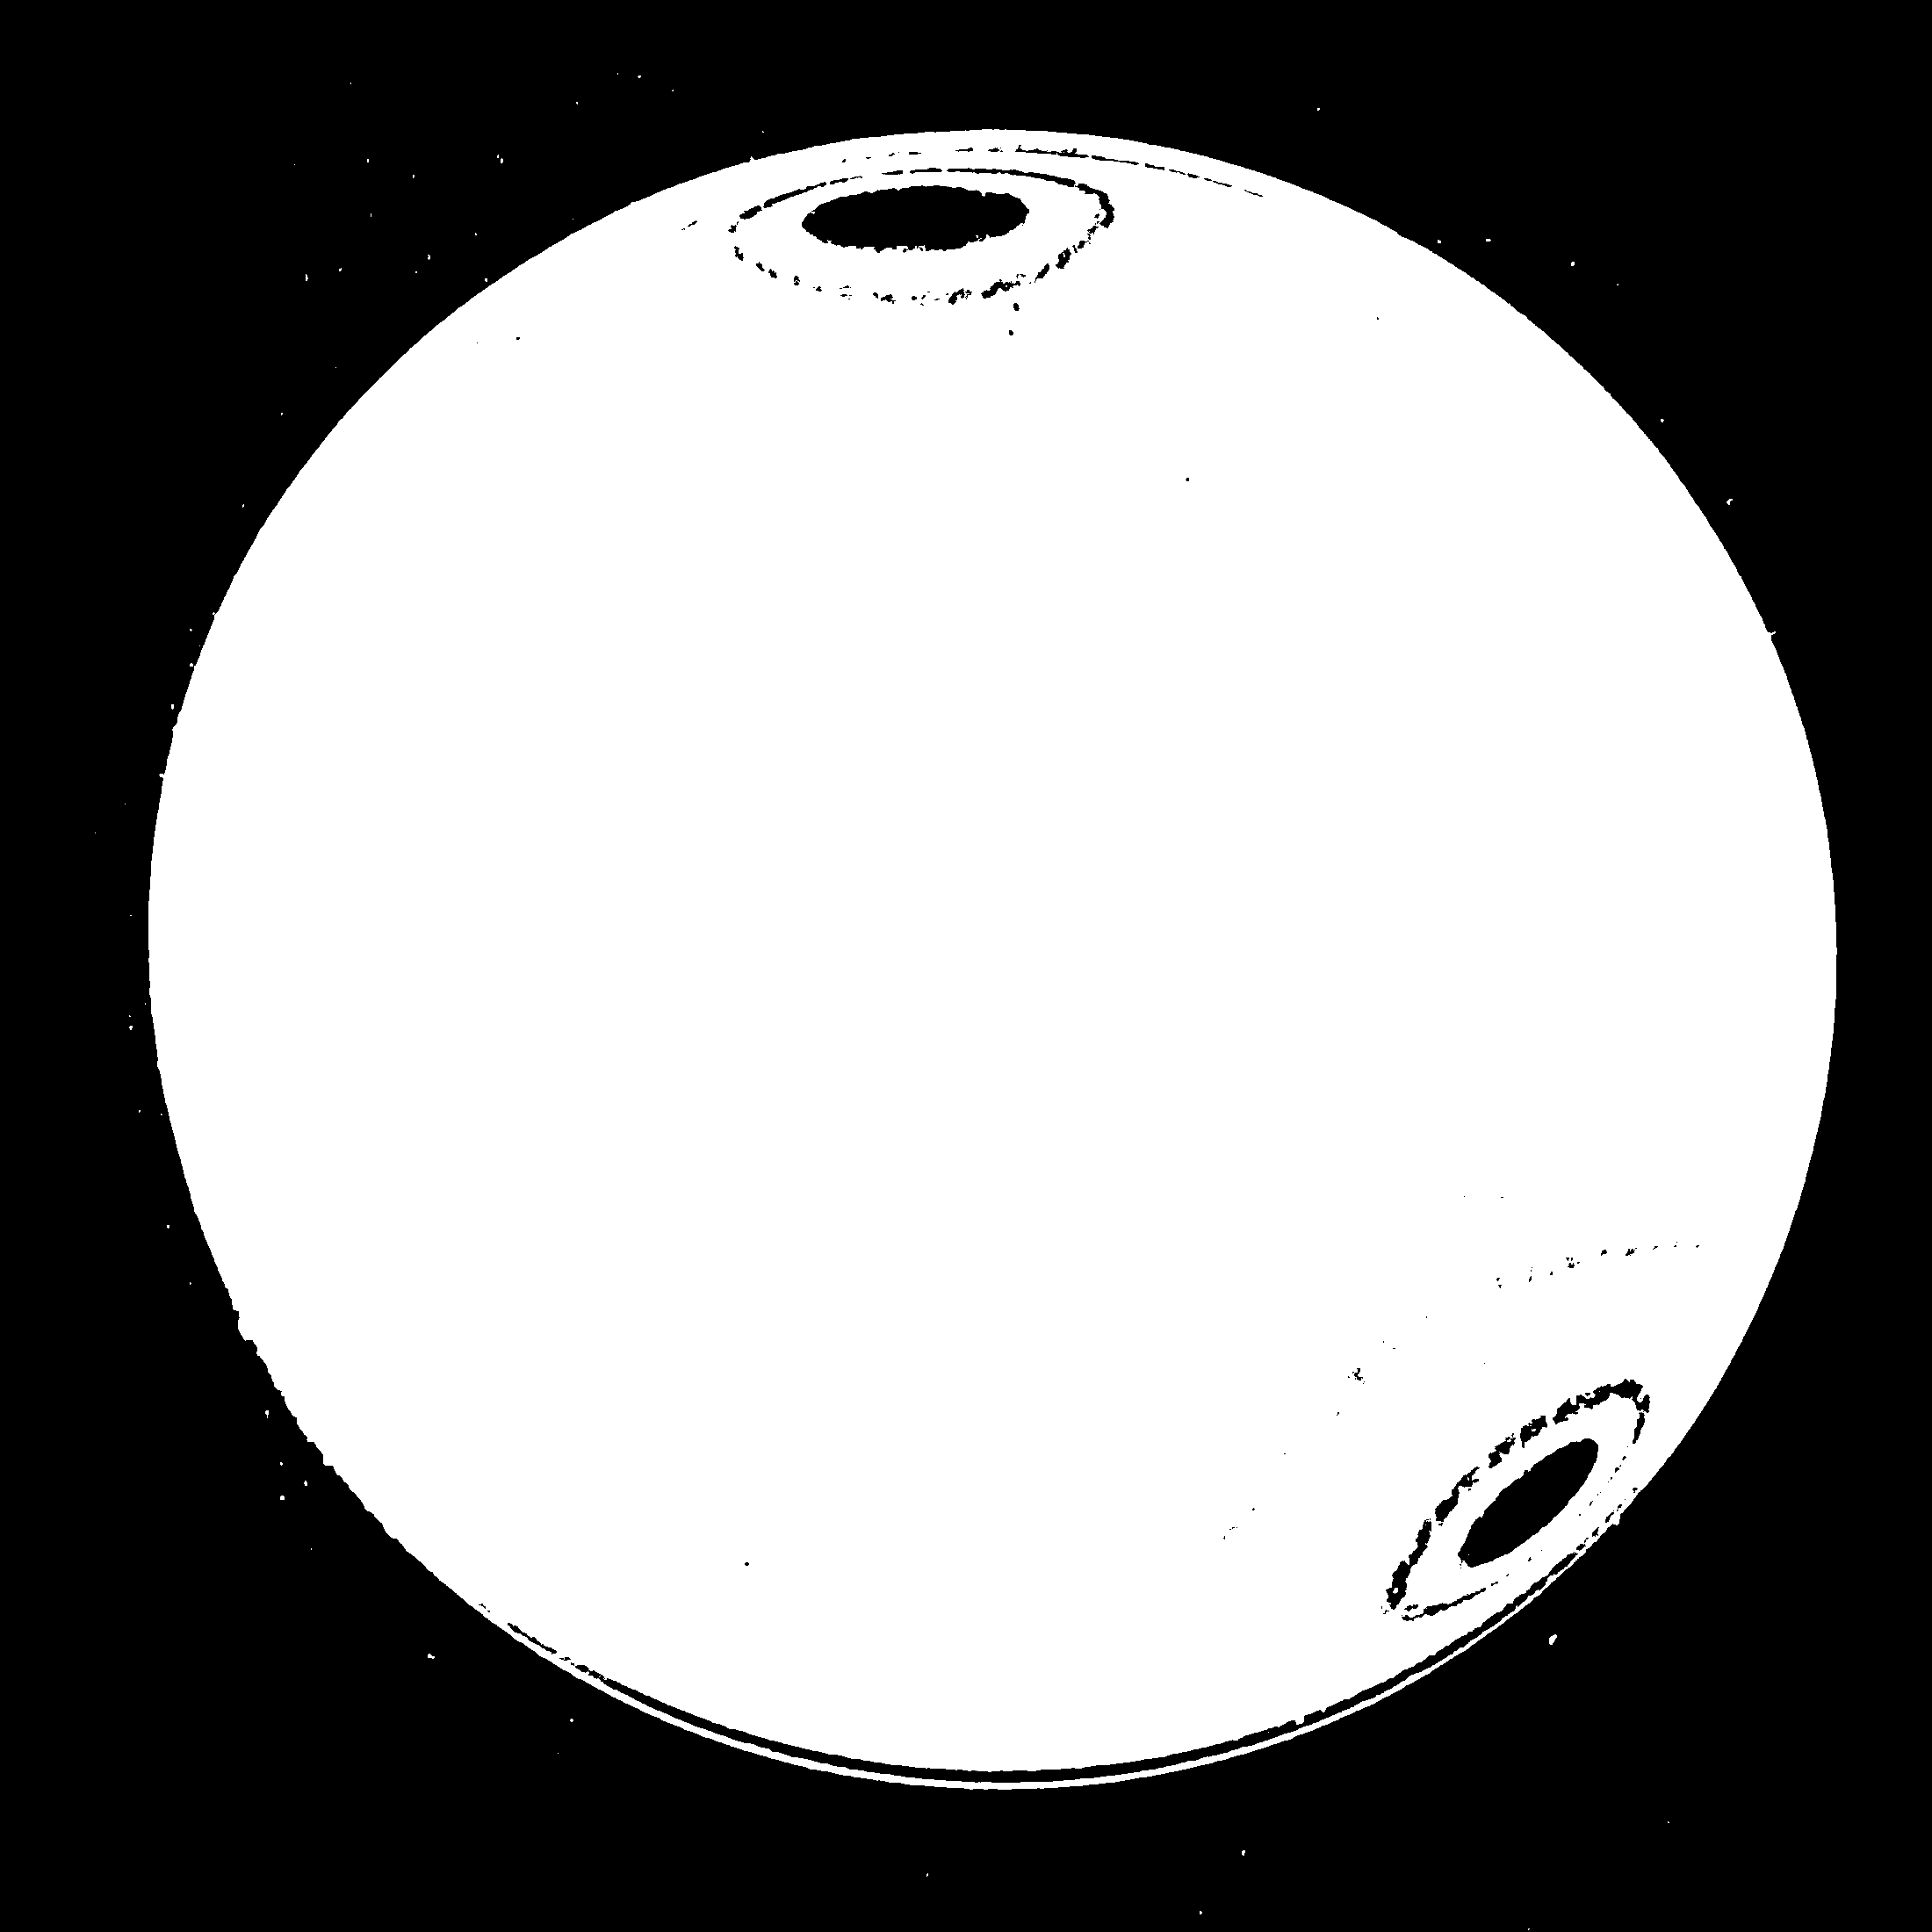
\includegraphics[width=\linewidth]{Images/Disks/Processed/acetone.png}
        \caption{Baseline Ethanol: Fiji analysis.}
        \label{fig:eth_fiji}
    \end{subfigure}
    
    \vspace{1em}
    
    % Pair 2: Plasma-Only
    \begin{subfigure}{0.45\linewidth}
        \centering
        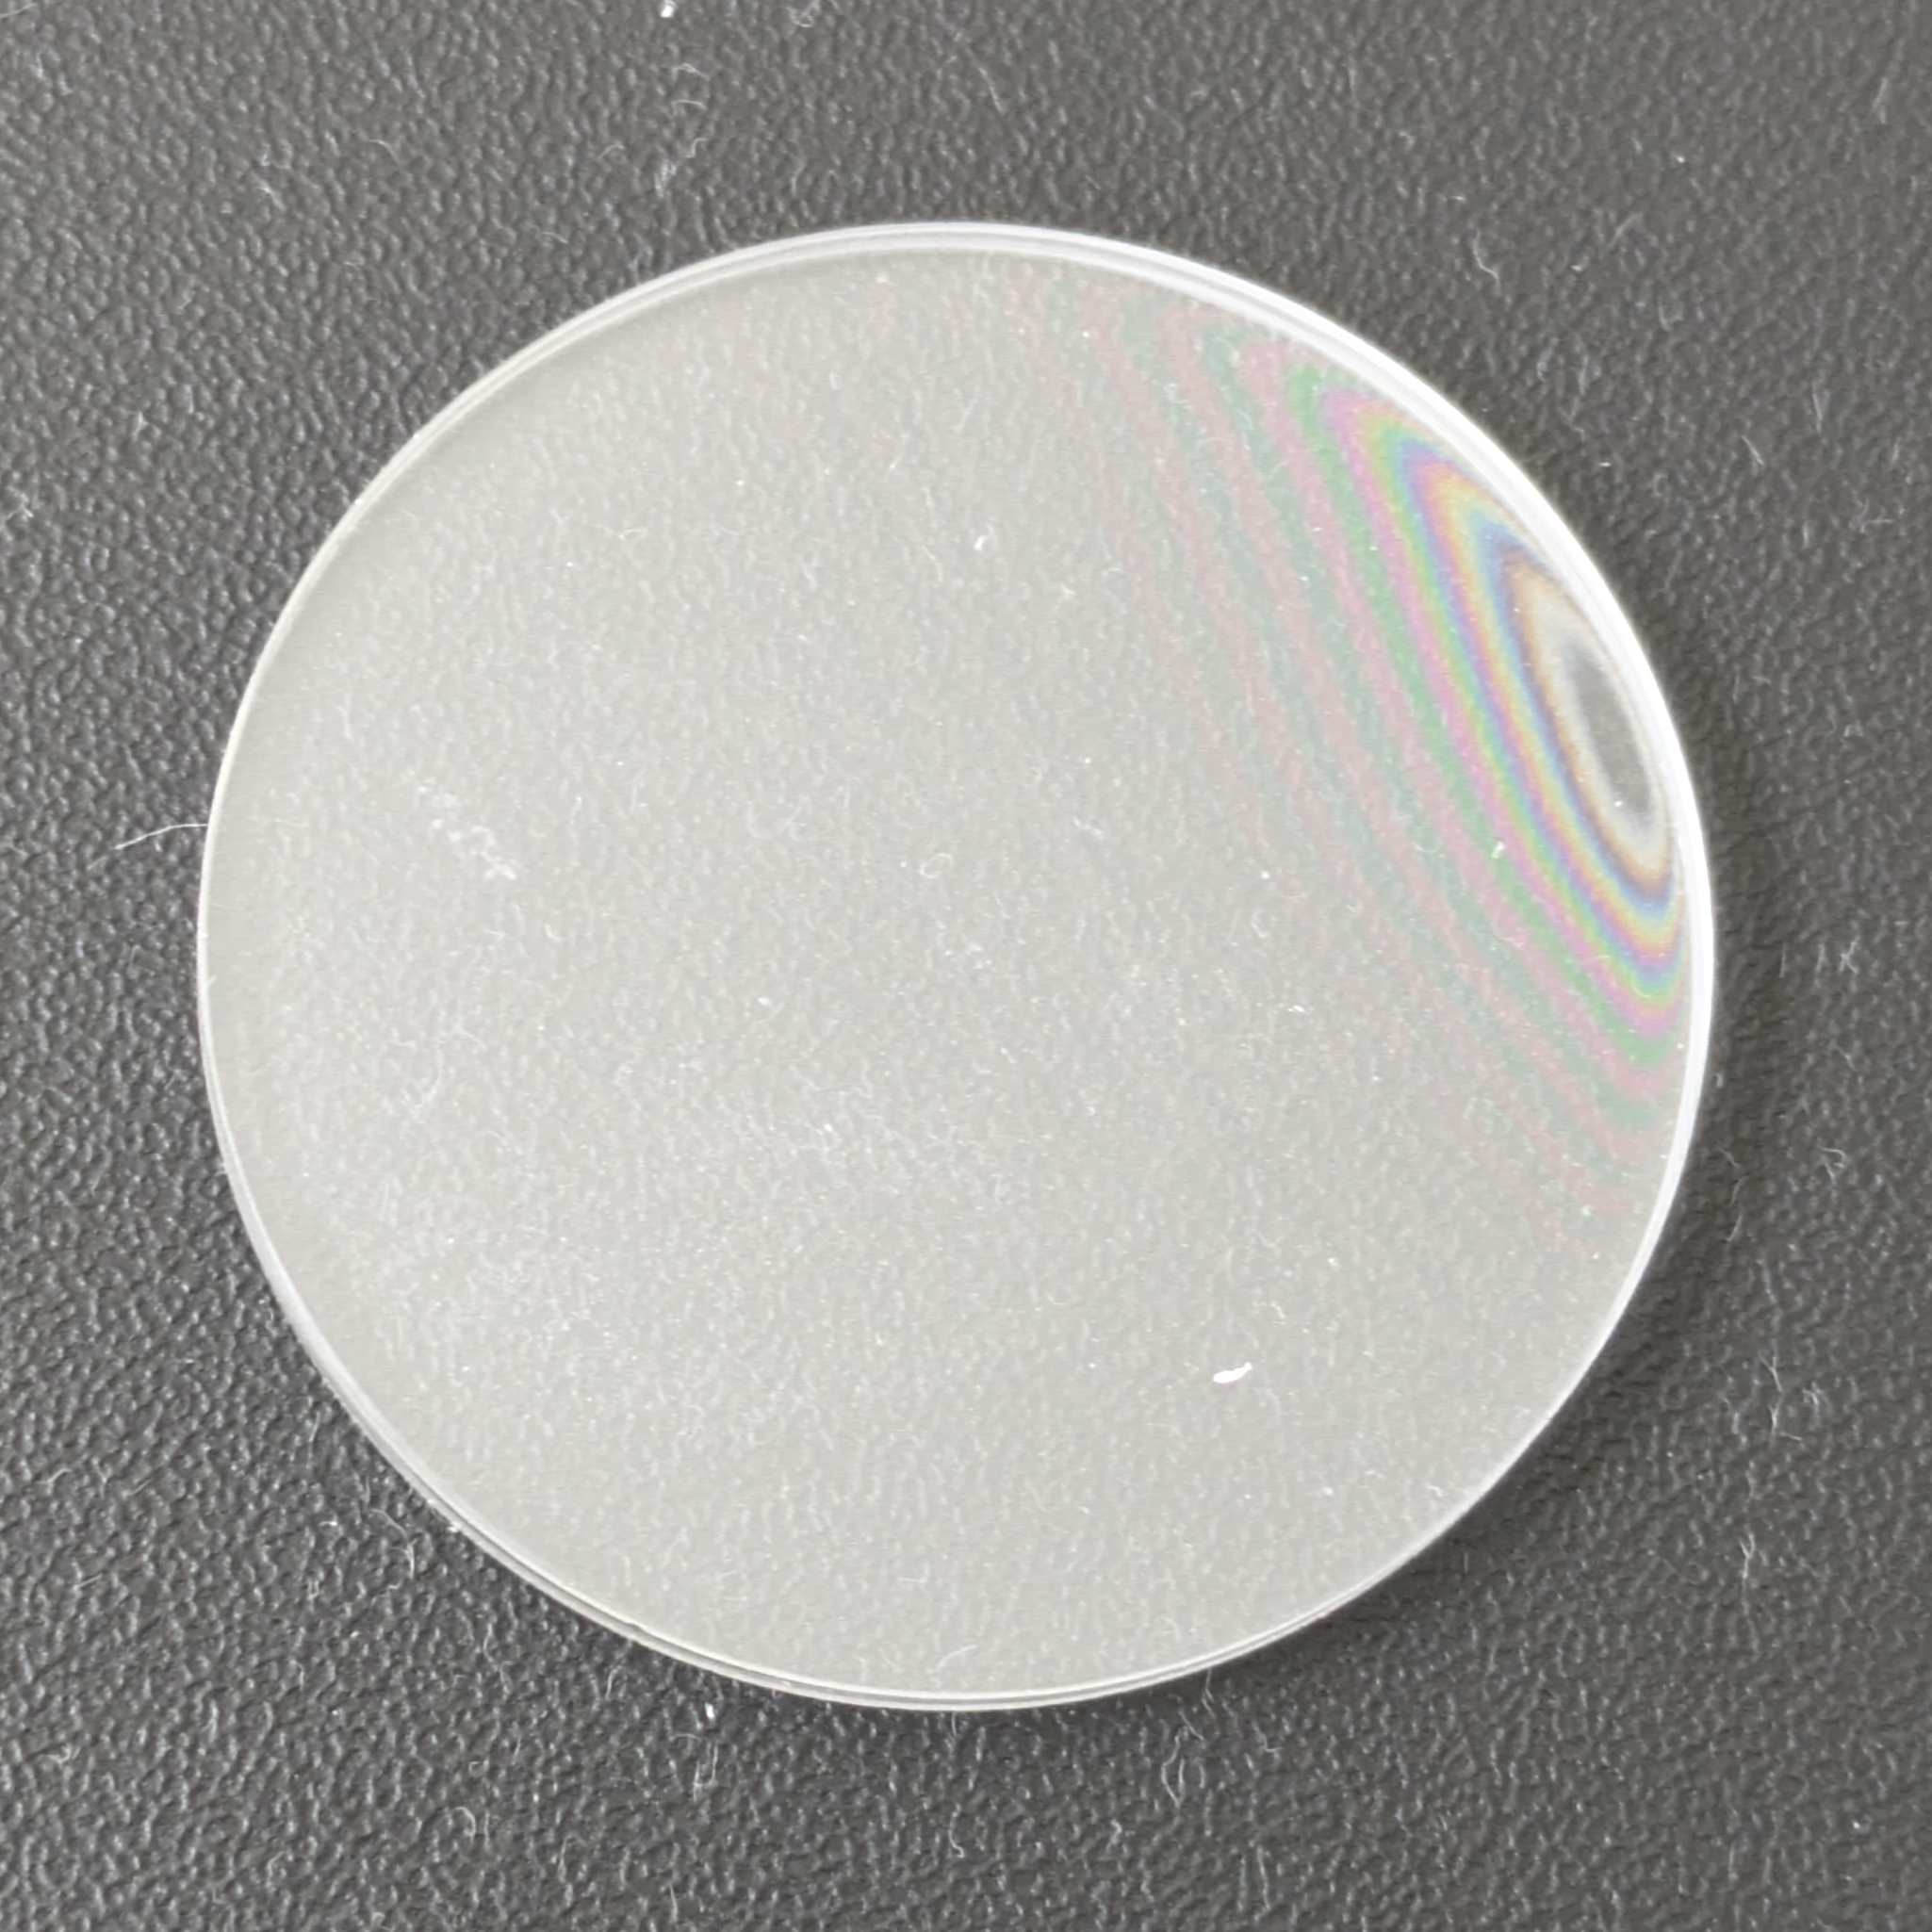
\includegraphics[width=\linewidth]{Images/Disks/Raw/plasma10.png}
        \caption{Plasma-Only: Raw photograph.}
        \label{fig:plasma_raw}
    \end{subfigure}
    \hfill
    \begin{subfigure}{0.45\linewidth}
        \centering
        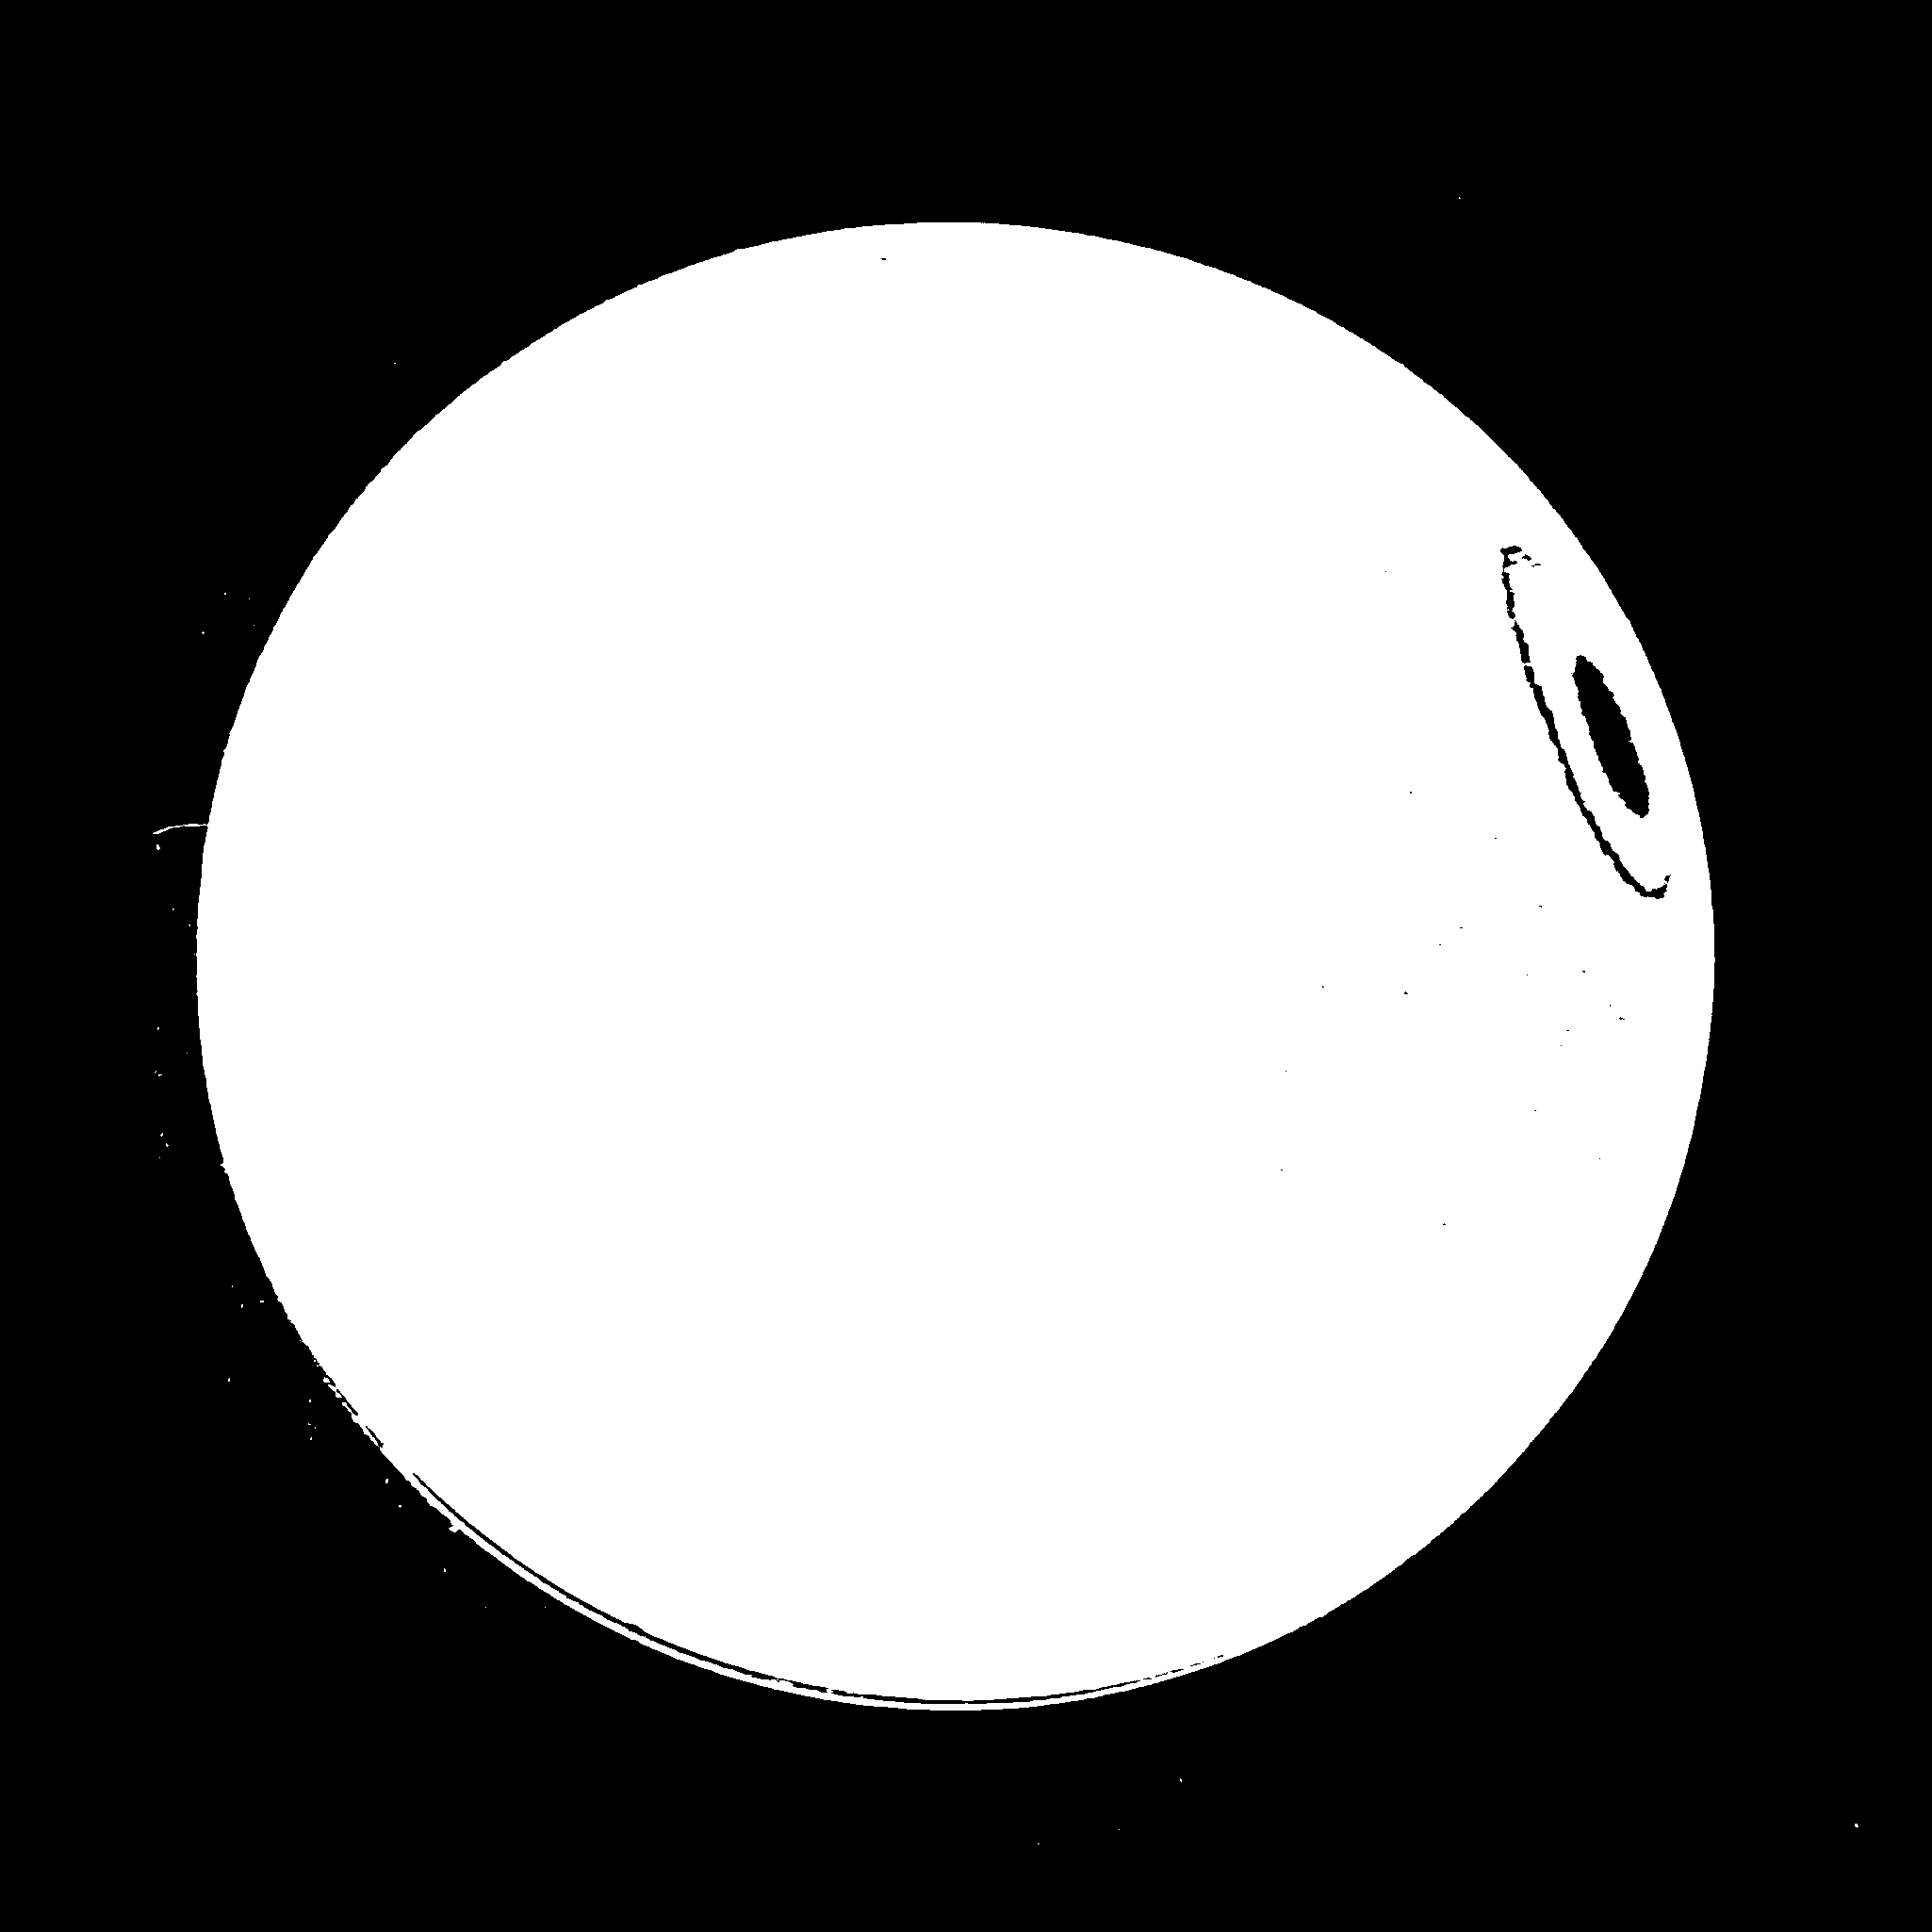
\includegraphics[width=\linewidth]{Images/Disks/Processed/plasma10.png}
        \caption{Plasma-Only: Fiji analysis.}
        \label{fig:plasma_fiji}
    \end{subfigure}
    \caption{Side-by-side bonding results (Part I). The left subfigures show
    the raw optical image of the bonded pair, while the right subfigures
    display the Fiji high-contrast binary map highlighting bonded regions
    (dark) and unbonded voids (bright).}
    \label{fig:bonding_results_1}
\end{figure}

\begin{figure}[htbp]
    \centering
    % Pair 3: Piranha Solution
    \begin{subfigure}{0.45\linewidth}
        \centering
        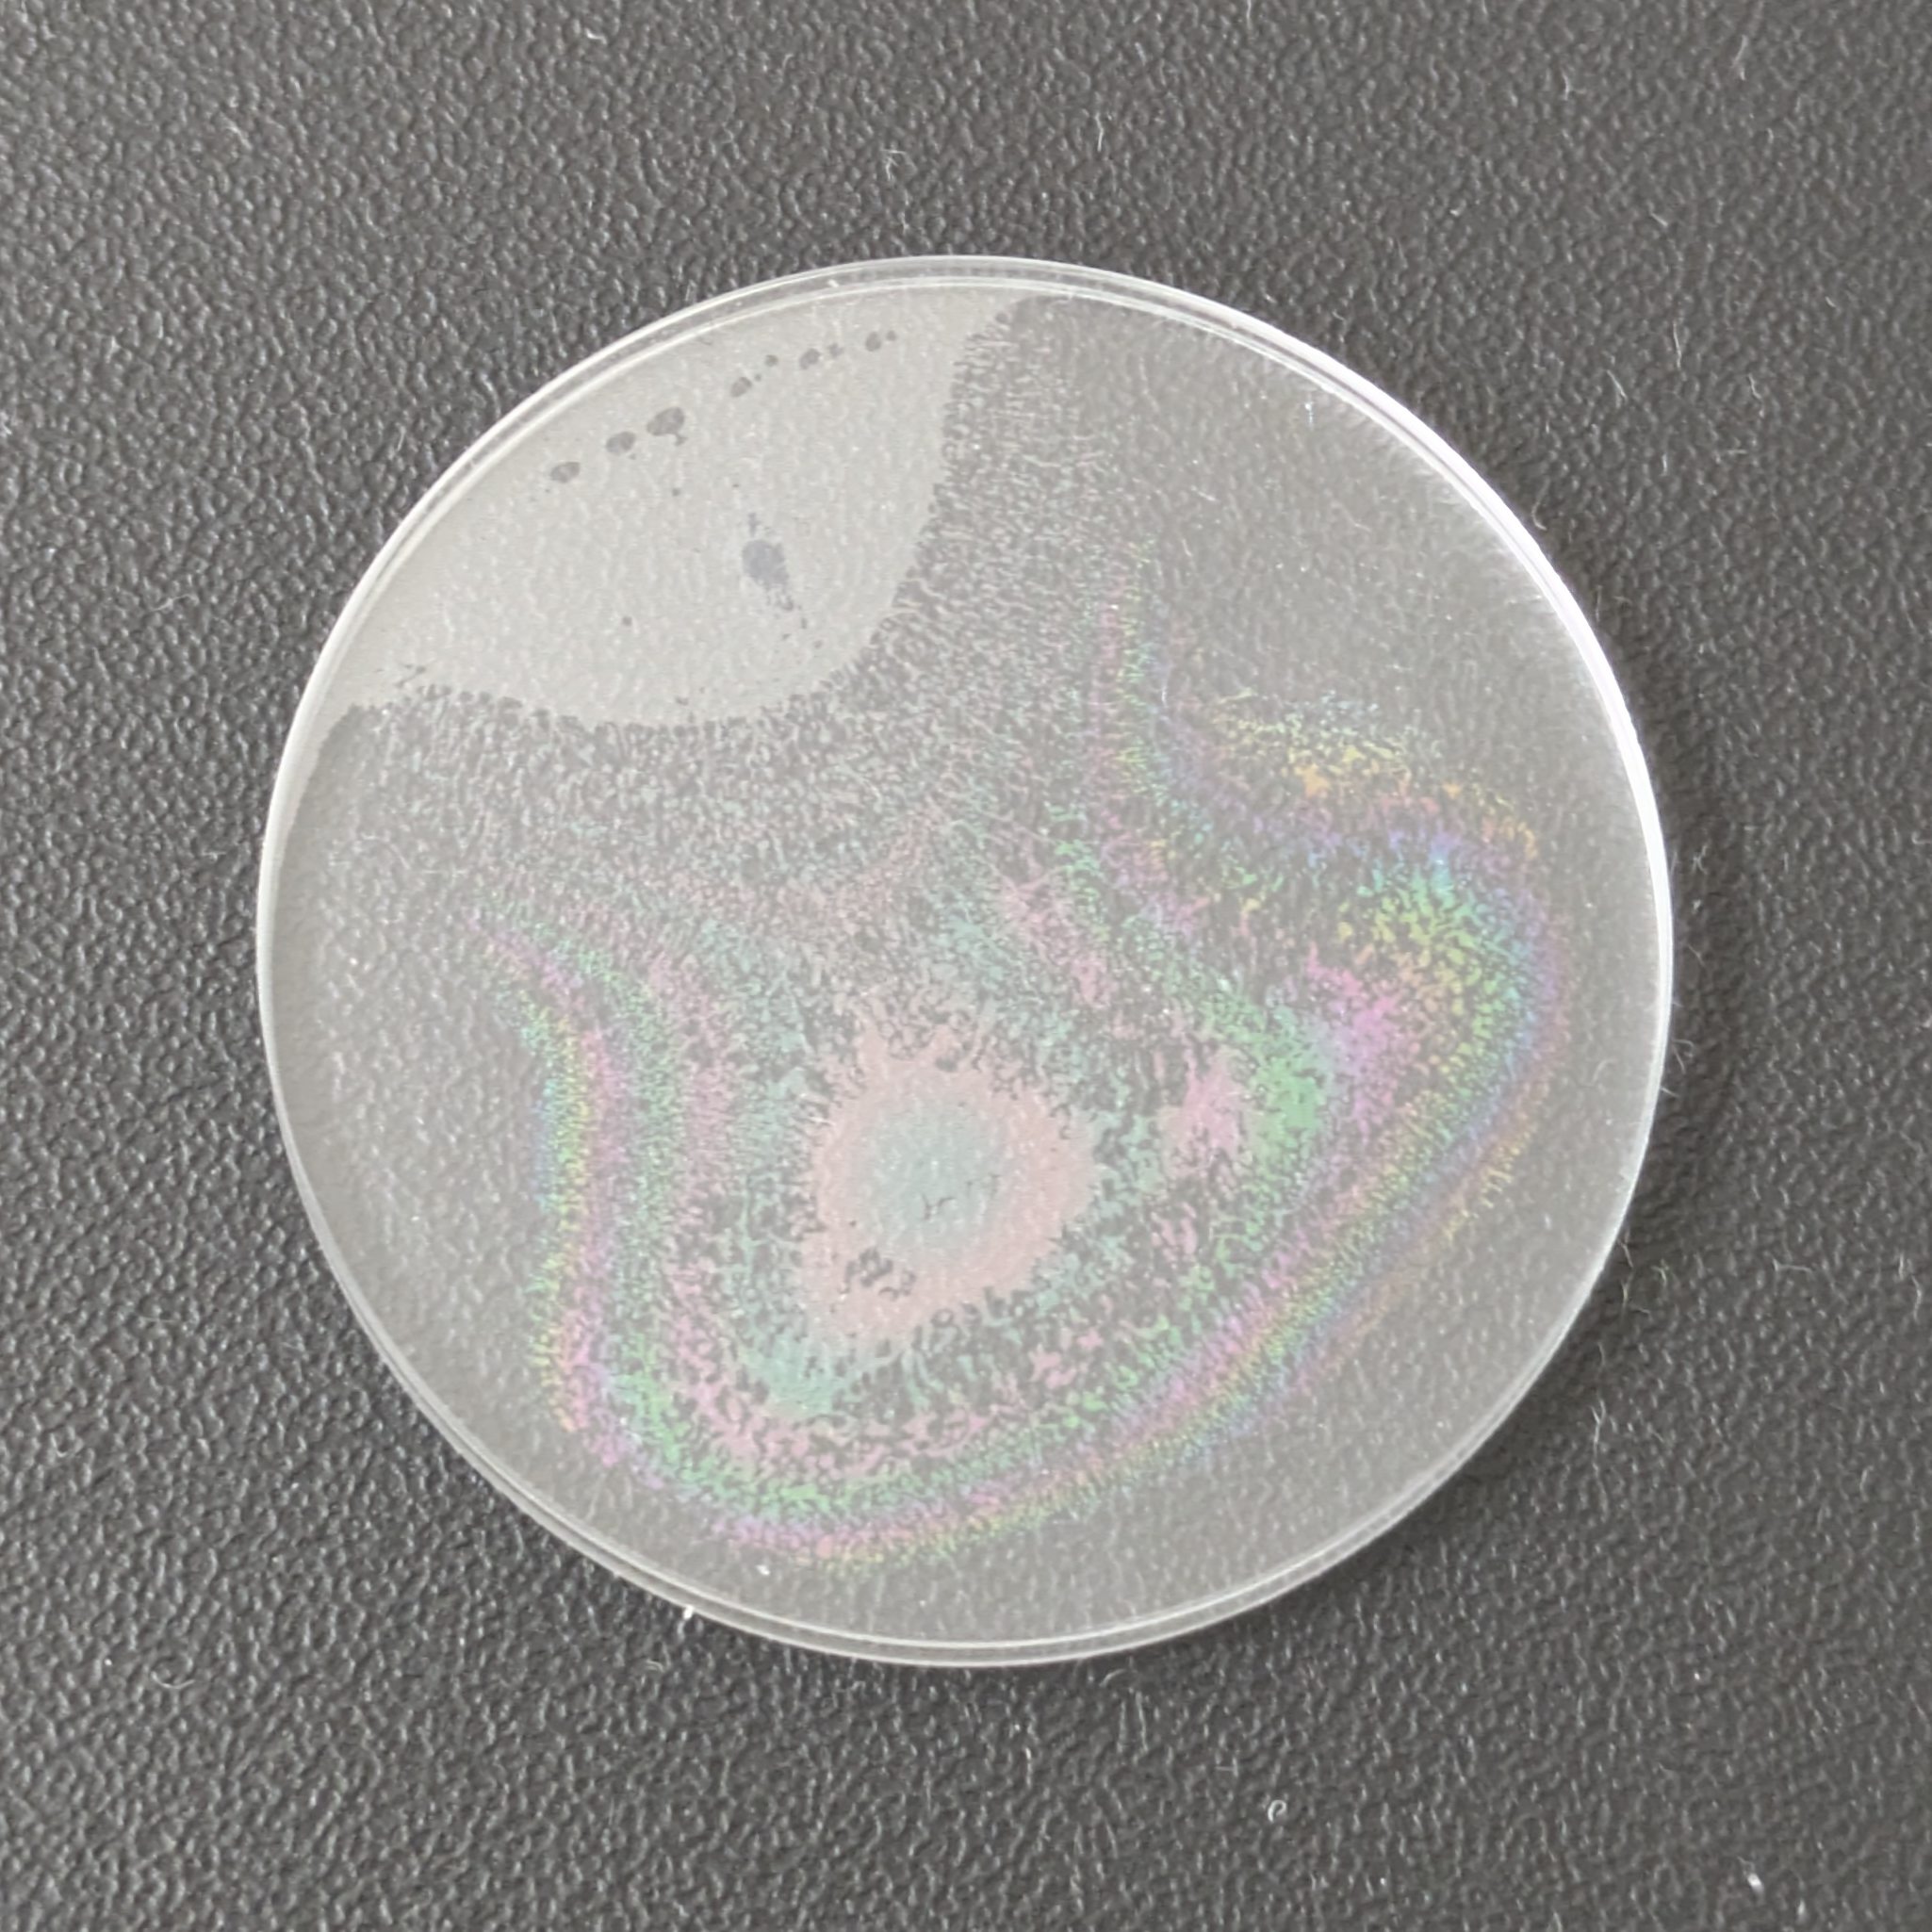
\includegraphics[width=\linewidth]{Images/Disks/Raw/piranha.png}
        \caption{Piranha Solution: Raw photograph.}
        \label{fig:piranha_raw}
    \end{subfigure}
    \hfill
    \begin{subfigure}{0.45\linewidth}
        \centering
        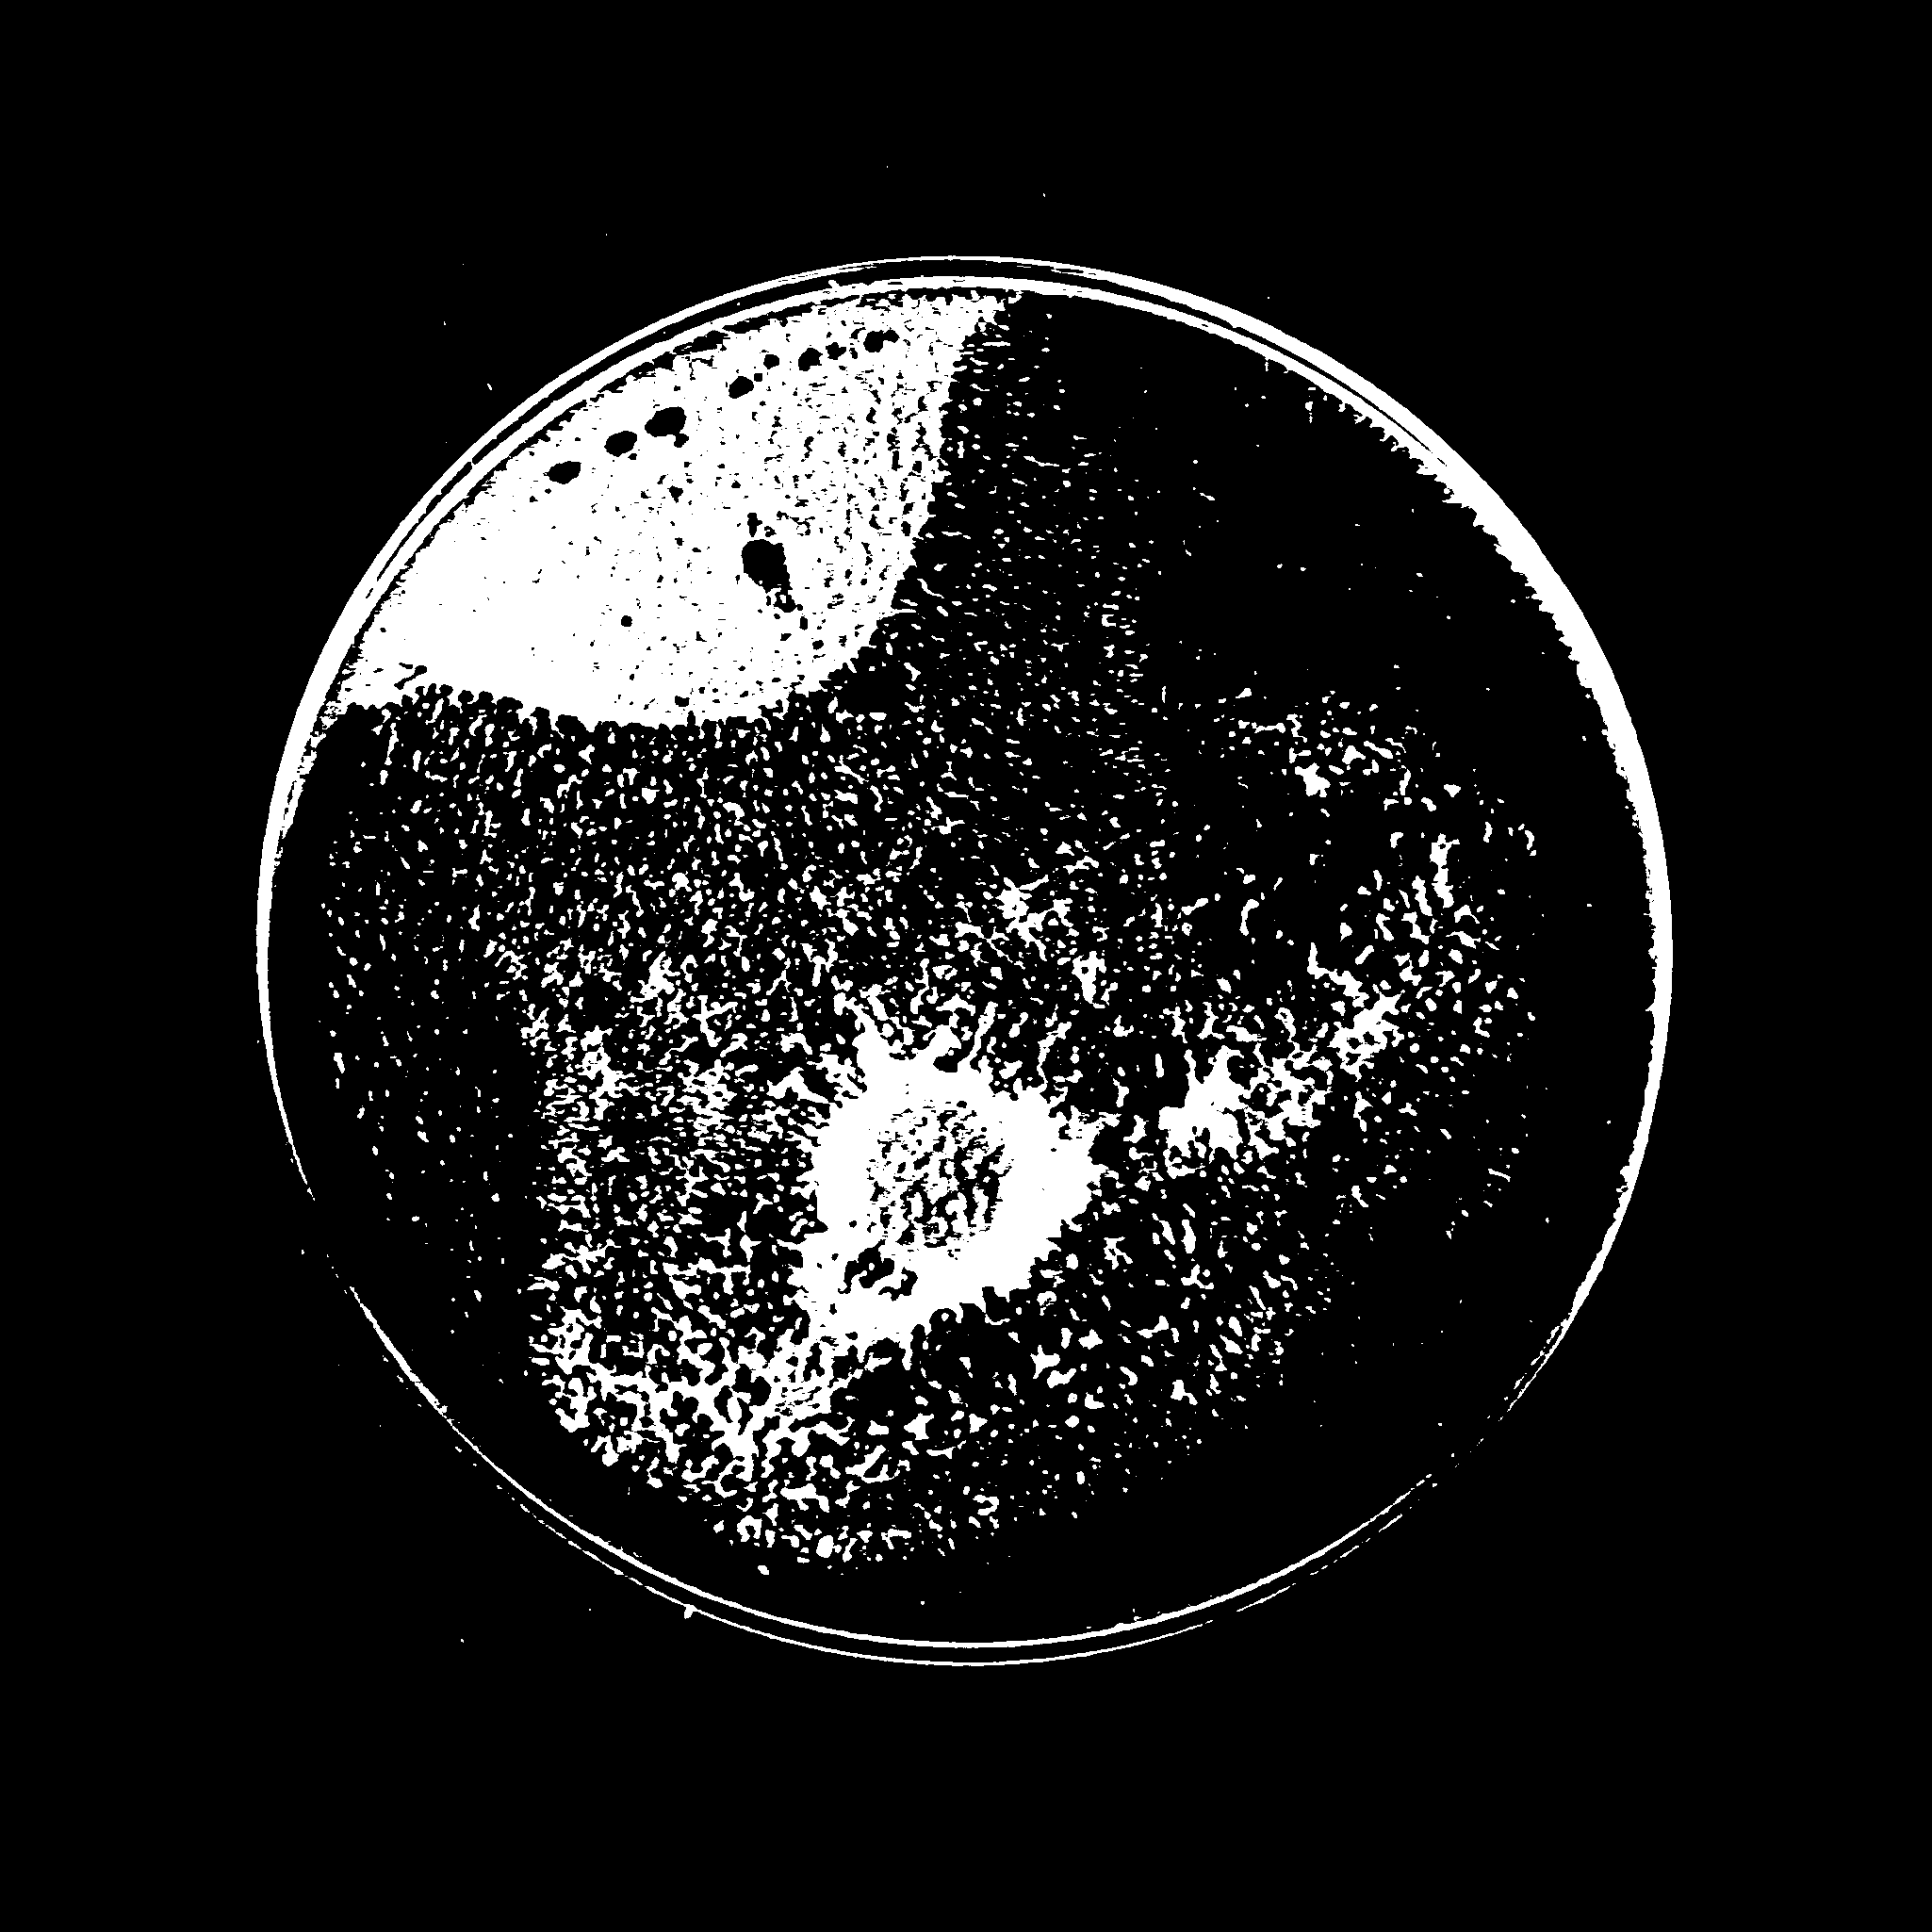
\includegraphics[width=\linewidth]{Images/Disks/Processed/piranha.png}
        \caption{Piranha Solution: Fiji analysis.}
        \label{fig:piranha_fiji}
    \end{subfigure}
    
    \vspace{1em}
    
    % Pair 4: RCA-1 + Piranha
    \begin{subfigure}{0.45\linewidth}
        \centering
        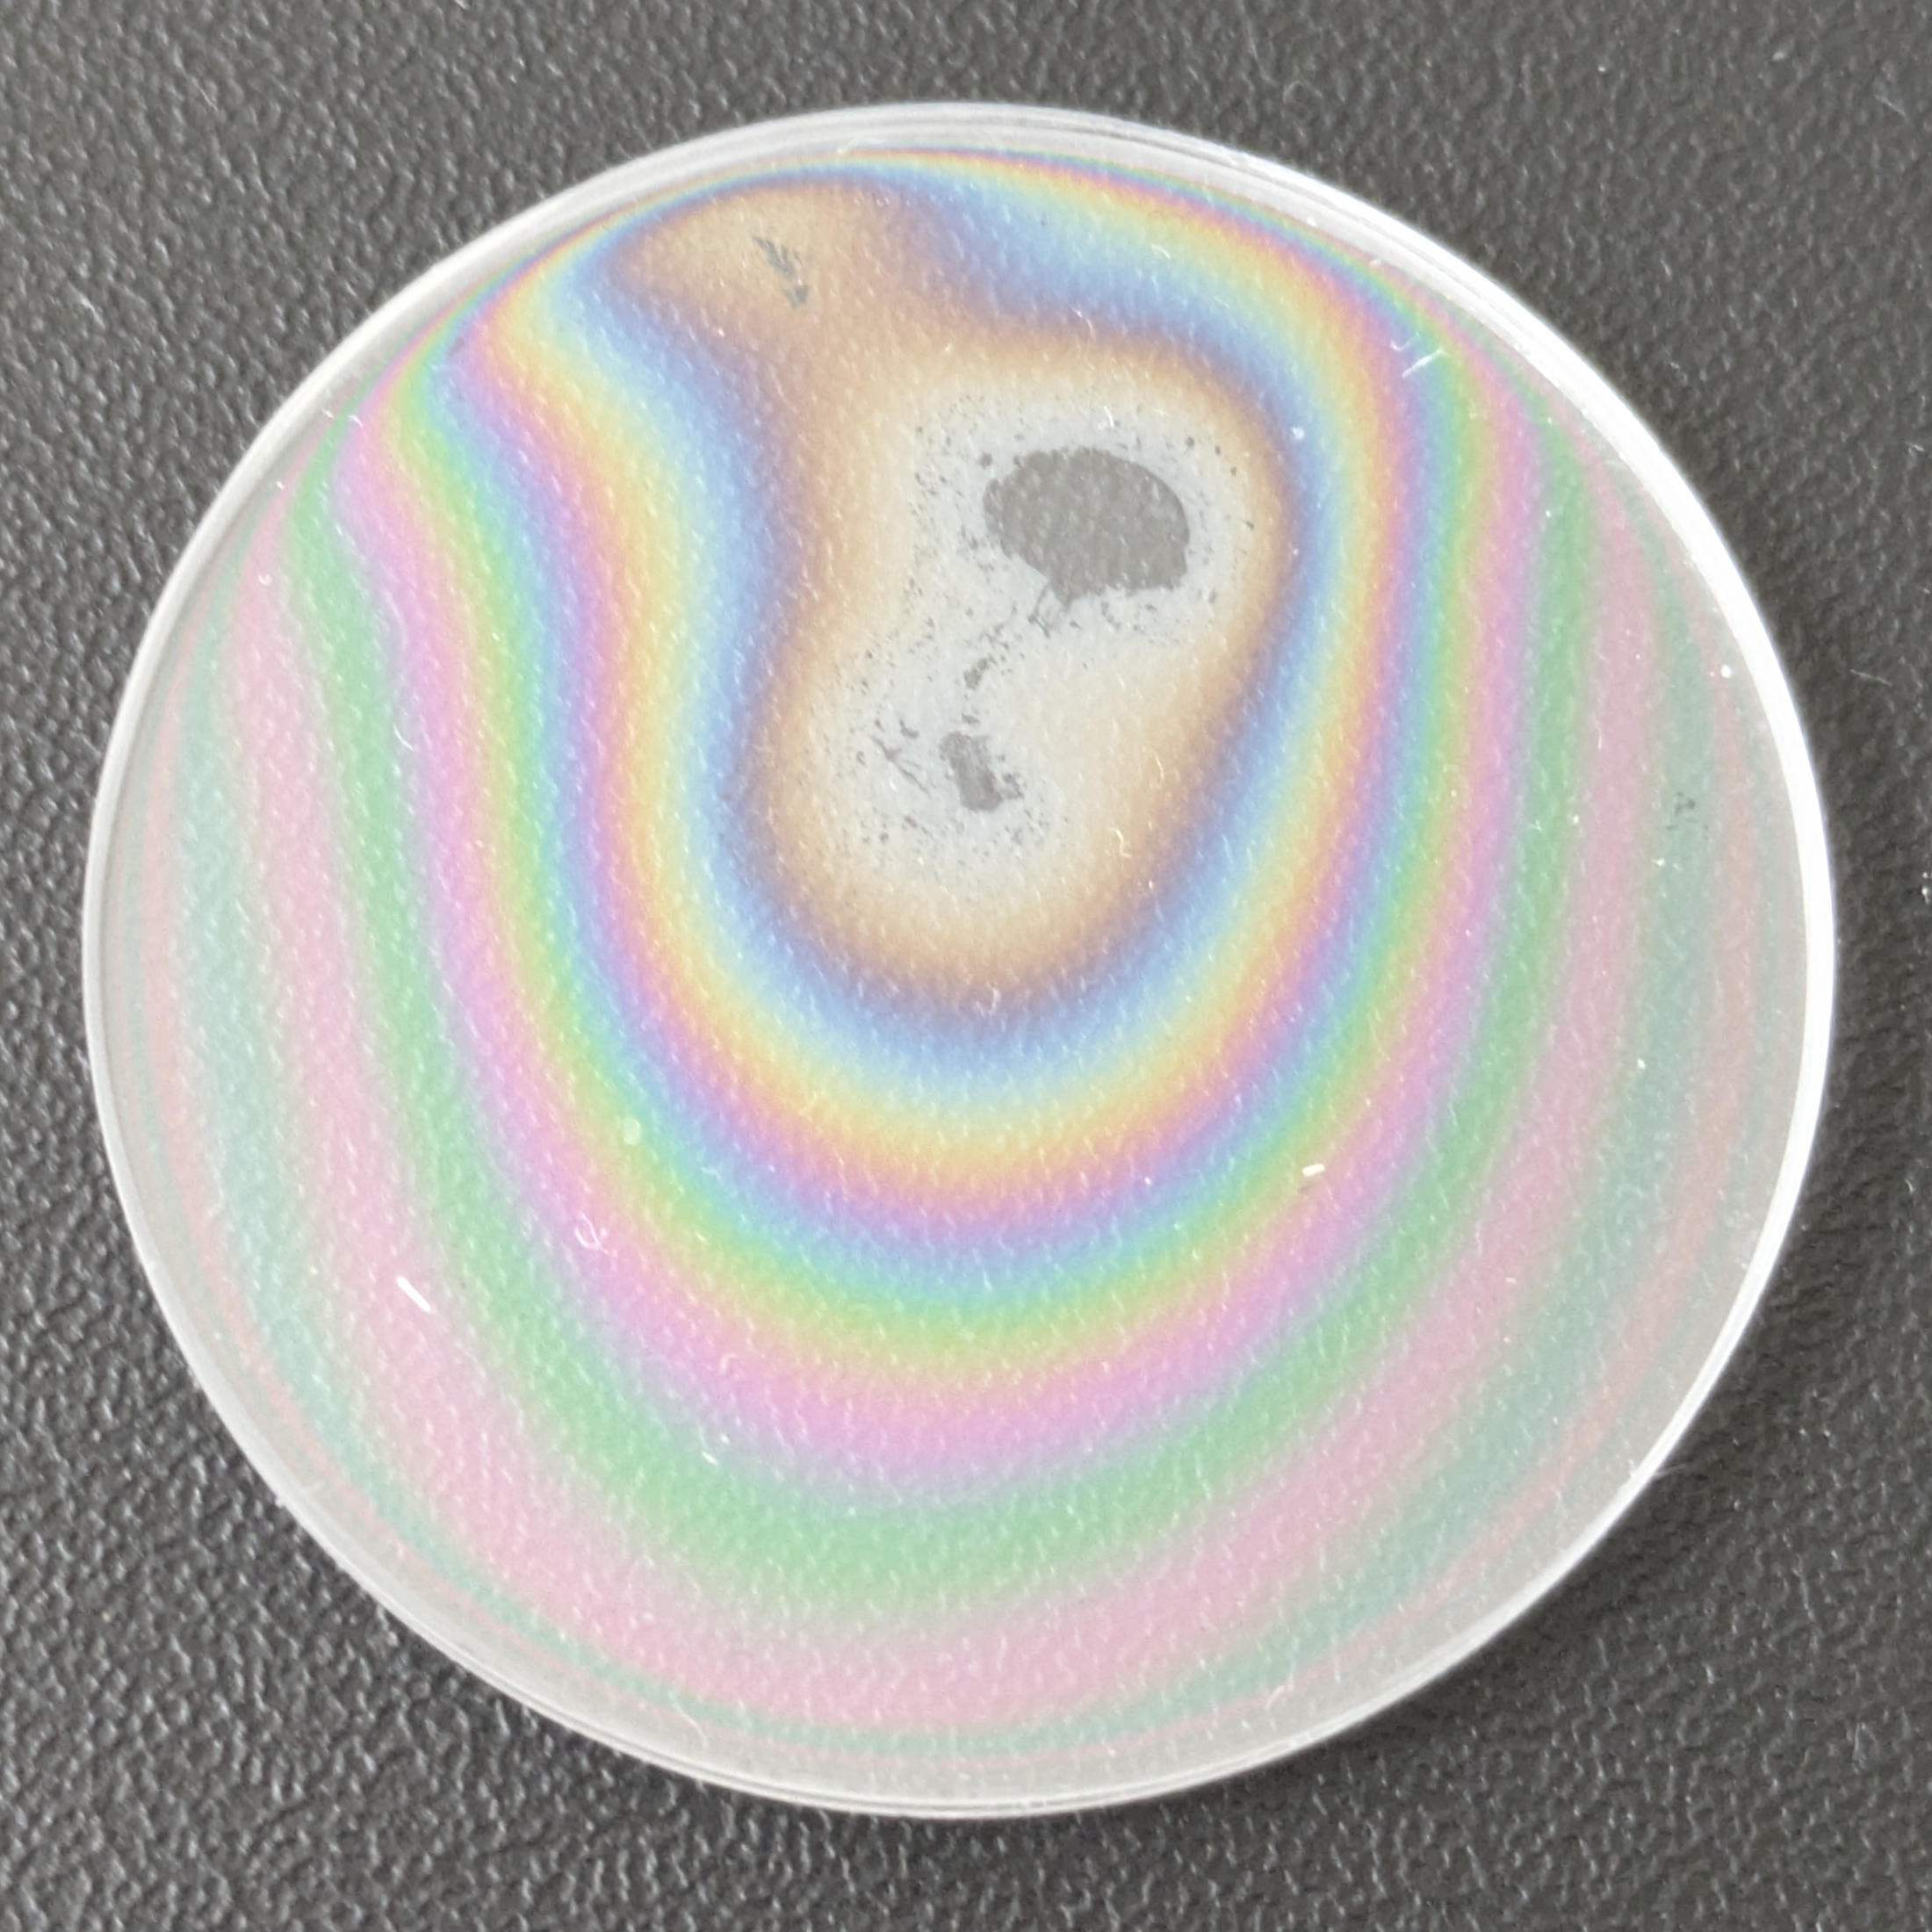
\includegraphics[width=\linewidth]{Images/Disks/Raw/rca_piranha.png}
        \caption{RCA-1 + Piranha: Raw photograph.}
        \label{fig:rca_raw}
    \end{subfigure}
    \hfill
    \begin{subfigure}{0.45\linewidth}
        \centering
        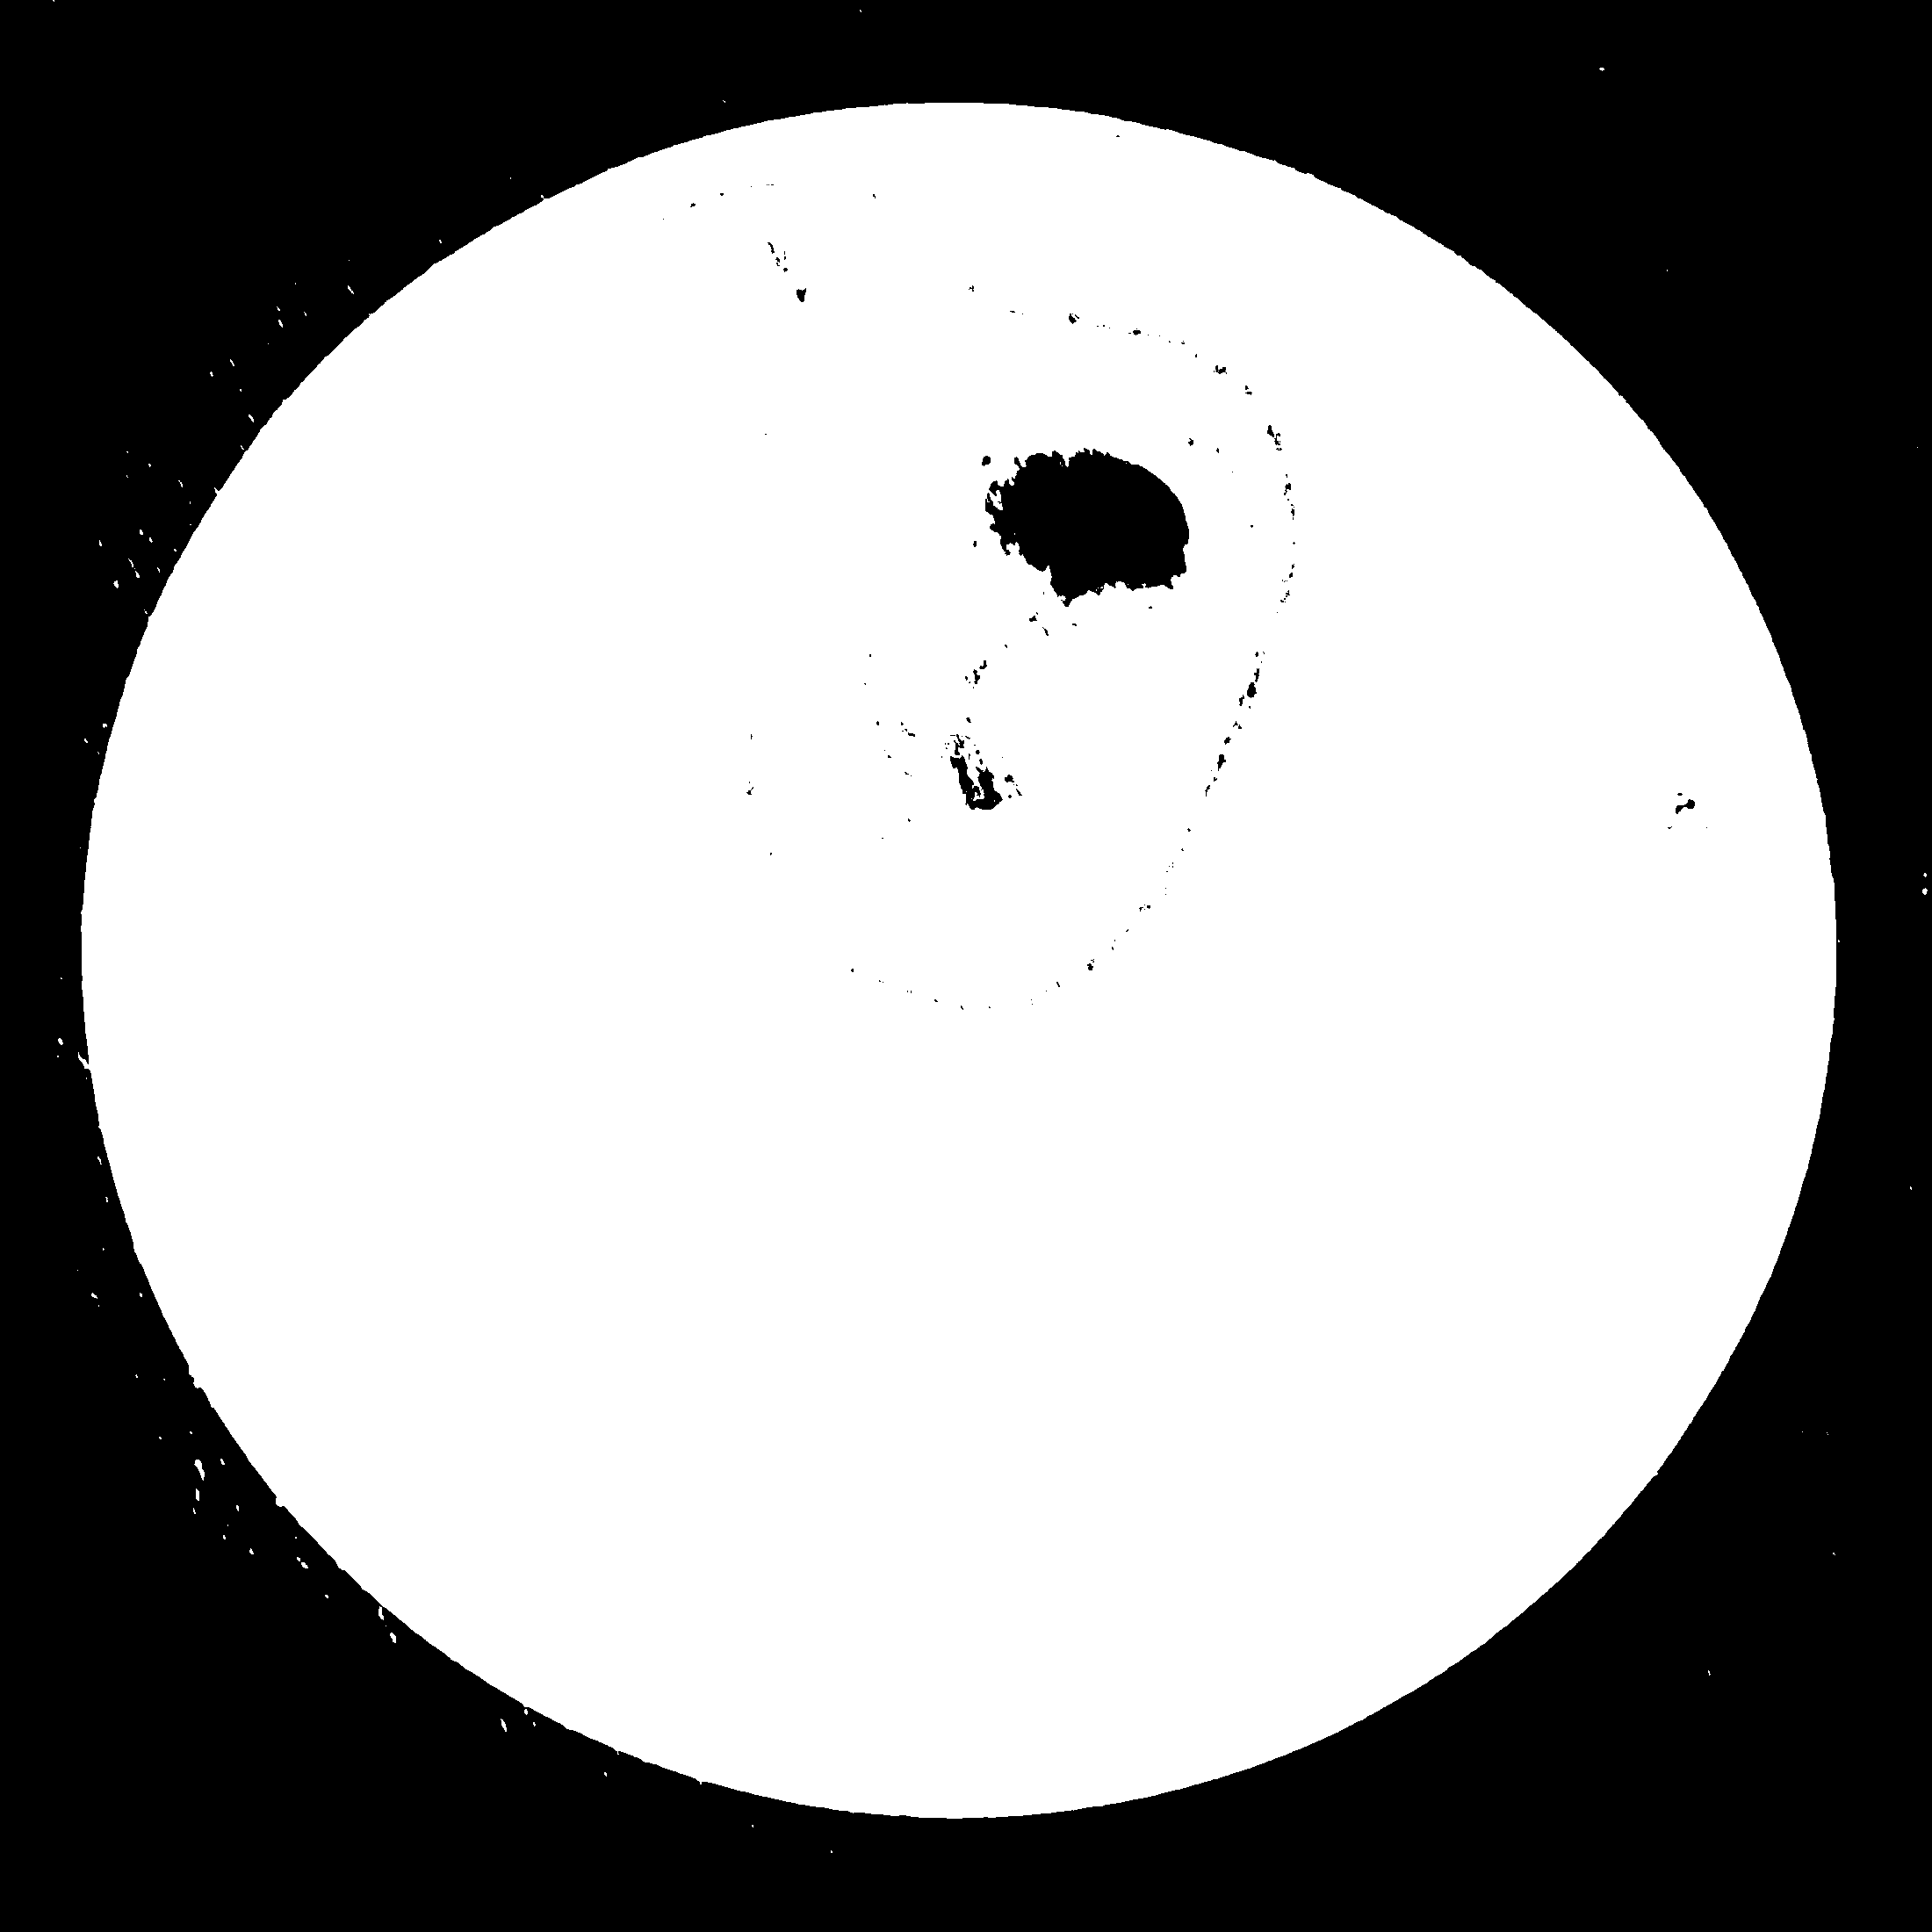
\includegraphics[width=\linewidth]{Images/Disks/Processed/rca_piranha.png}
        \caption{RCA-1 + Piranha: Fiji analysis.}
        \label{fig:rca_fiji}
    \end{subfigure}
    \caption{Side-by-side bonding results (Part II). Left: raw optical
    photographs. Right: corresponding Fiji binary processed maps.}
    \label{fig:bonding_results_2}
\end{figure}

\subsection{Tensile Testing and Mechanical Characterization}
To evaluate the mechanical robustness of the optical contact bonds, a series
of tensile tests were performed on the successfully bonded pairs. Evaluating
the tensile strength is critical to ensure that the sealed vapor cells can
withstand internal pressure variations and mechanical shocks during operation.

To properly grip the fused silica disks without introducing parasitic shear
stresses or scratching the delicate glass surfaces, custom mounting fixtures
were designed and manufactured using 3D printing (Figure~\ref{fig:3d_fixture}).
These polymeric holders provided a uniform stress distribution across the
sample area during the pulling phase.

\begin{figure}[htbp]
    \centering
    
\includegraphics[width=0.5\linewidth]{Images/placeholder.png}
    \caption{Custom 3D-printed fixture designed to securely hold the fused
    silica disks during the tensile test without inducing shear stress.}
    \label{fig:3d_fixture}
\end{figure}

The assembled samples were then mounted into a dedicated tensile testing
machine (Figure~\ref{fig:tensile_setup}). A progressively increasing normal
force was applied perpendicular to the bonded interface until mechanical
failure (debonding or bulk fracture) occurred. The peak force recorded at the
moment of failure was utilized to calculate the maximum supported pressure
for each bonding configuration.

\begin{figure}[htbp]
    \centering
    
\includegraphics[width=0.6\linewidth]{Images/placeholder.png}
    \caption{Experimental setup for the tensile test, showing the bonded
    fused silica disks mounted within the 3D-printed fixtures and attached
    to the testing machine.}
    \label{fig:tensile_setup}
\end{figure}

Table~\ref{tab:tensile_results} summarizes the mechanical performance of the
bonded pairs across the different activation protocols. The effective bonded
area percentages, extracted from the prior Fiji (ImageJ) optical analysis,
are directly correlated with the maximum supported pressure measured during
the tensile tests.

\begin{table}[htbp]
    \centering
    \caption{Correlation between the surface activation procedure, the
    effective bonded area, and the maximum supported pressure.}
    \label{tab:tensile_results}
    \begin{tabular}{lcc}
        \toprule
        \textbf{Procedure} & \textbf{Bonded} & \textbf{Supported} \\
                           & \textbf{Area (\%)} & \textbf{Pressure (MPa)} \\
        \midrule
        Baseline Ethanol             & [PLACEHOLDER] & [PLACEHOLDER] \\
        Plasma (\SI{5}{\minute})     & [PLACEHOLDER] & [PLACEHOLDER] \\
        Plasma (\SI{10}{\minute})    & [PLACEHOLDER] & [PLACEHOLDER] \\
        Piranha (\SI{20}{\minute})   & [PLACEHOLDER] & [PLACEHOLDER] \\
        RCA-1 + Piranha              & [PLACEHOLDER] & [PLACEHOLDER] \\
        Piranha + Plasma             & [PLACEHOLDER] & [PLACEHOLDER] \\
        \bottomrule
    \end{tabular}
\end{table}